% Options for packages loaded elsewhere
\PassOptionsToPackage{unicode}{hyperref}
\PassOptionsToPackage{hyphens}{url}
\PassOptionsToPackage{dvipsnames,svgnames,x11names}{xcolor}
%
\documentclass[
  letterpaper,
  DIV=11,
  numbers=noendperiod,
  oneside]{scrartcl}

\usepackage{amsmath,amssymb}
\usepackage{iftex}
\ifPDFTeX
  \usepackage[T1]{fontenc}
  \usepackage[utf8]{inputenc}
  \usepackage{textcomp} % provide euro and other symbols
\else % if luatex or xetex
  \usepackage{unicode-math}
  \defaultfontfeatures{Scale=MatchLowercase}
  \defaultfontfeatures[\rmfamily]{Ligatures=TeX,Scale=1}
\fi
\usepackage{lmodern}
\ifPDFTeX\else  
    % xetex/luatex font selection
\fi
% Use upquote if available, for straight quotes in verbatim environments
\IfFileExists{upquote.sty}{\usepackage{upquote}}{}
\IfFileExists{microtype.sty}{% use microtype if available
  \usepackage[]{microtype}
  \UseMicrotypeSet[protrusion]{basicmath} % disable protrusion for tt fonts
}{}
\makeatletter
\@ifundefined{KOMAClassName}{% if non-KOMA class
  \IfFileExists{parskip.sty}{%
    \usepackage{parskip}
  }{% else
    \setlength{\parindent}{0pt}
    \setlength{\parskip}{6pt plus 2pt minus 1pt}}
}{% if KOMA class
  \KOMAoptions{parskip=half}}
\makeatother
\usepackage{xcolor}
\usepackage[left=1in,marginparwidth=2.0666666666667in,textwidth=4.1333333333333in,marginparsep=0.3in]{geometry}
\setlength{\emergencystretch}{3em} % prevent overfull lines
\setcounter{secnumdepth}{-\maxdimen} % remove section numbering
% Make \paragraph and \subparagraph free-standing
\makeatletter
\ifx\paragraph\undefined\else
  \let\oldparagraph\paragraph
  \renewcommand{\paragraph}{
    \@ifstar
      \xxxParagraphStar
      \xxxParagraphNoStar
  }
  \newcommand{\xxxParagraphStar}[1]{\oldparagraph*{#1}\mbox{}}
  \newcommand{\xxxParagraphNoStar}[1]{\oldparagraph{#1}\mbox{}}
\fi
\ifx\subparagraph\undefined\else
  \let\oldsubparagraph\subparagraph
  \renewcommand{\subparagraph}{
    \@ifstar
      \xxxSubParagraphStar
      \xxxSubParagraphNoStar
  }
  \newcommand{\xxxSubParagraphStar}[1]{\oldsubparagraph*{#1}\mbox{}}
  \newcommand{\xxxSubParagraphNoStar}[1]{\oldsubparagraph{#1}\mbox{}}
\fi
\makeatother

\usepackage{color}
\usepackage{fancyvrb}
\newcommand{\VerbBar}{|}
\newcommand{\VERB}{\Verb[commandchars=\\\{\}]}
\DefineVerbatimEnvironment{Highlighting}{Verbatim}{commandchars=\\\{\}}
% Add ',fontsize=\small' for more characters per line
\usepackage{framed}
\definecolor{shadecolor}{RGB}{241,243,245}
\newenvironment{Shaded}{\begin{snugshade}}{\end{snugshade}}
\newcommand{\AlertTok}[1]{\textcolor[rgb]{0.68,0.00,0.00}{#1}}
\newcommand{\AnnotationTok}[1]{\textcolor[rgb]{0.37,0.37,0.37}{#1}}
\newcommand{\AttributeTok}[1]{\textcolor[rgb]{0.40,0.45,0.13}{#1}}
\newcommand{\BaseNTok}[1]{\textcolor[rgb]{0.68,0.00,0.00}{#1}}
\newcommand{\BuiltInTok}[1]{\textcolor[rgb]{0.00,0.23,0.31}{#1}}
\newcommand{\CharTok}[1]{\textcolor[rgb]{0.13,0.47,0.30}{#1}}
\newcommand{\CommentTok}[1]{\textcolor[rgb]{0.37,0.37,0.37}{#1}}
\newcommand{\CommentVarTok}[1]{\textcolor[rgb]{0.37,0.37,0.37}{\textit{#1}}}
\newcommand{\ConstantTok}[1]{\textcolor[rgb]{0.56,0.35,0.01}{#1}}
\newcommand{\ControlFlowTok}[1]{\textcolor[rgb]{0.00,0.23,0.31}{\textbf{#1}}}
\newcommand{\DataTypeTok}[1]{\textcolor[rgb]{0.68,0.00,0.00}{#1}}
\newcommand{\DecValTok}[1]{\textcolor[rgb]{0.68,0.00,0.00}{#1}}
\newcommand{\DocumentationTok}[1]{\textcolor[rgb]{0.37,0.37,0.37}{\textit{#1}}}
\newcommand{\ErrorTok}[1]{\textcolor[rgb]{0.68,0.00,0.00}{#1}}
\newcommand{\ExtensionTok}[1]{\textcolor[rgb]{0.00,0.23,0.31}{#1}}
\newcommand{\FloatTok}[1]{\textcolor[rgb]{0.68,0.00,0.00}{#1}}
\newcommand{\FunctionTok}[1]{\textcolor[rgb]{0.28,0.35,0.67}{#1}}
\newcommand{\ImportTok}[1]{\textcolor[rgb]{0.00,0.46,0.62}{#1}}
\newcommand{\InformationTok}[1]{\textcolor[rgb]{0.37,0.37,0.37}{#1}}
\newcommand{\KeywordTok}[1]{\textcolor[rgb]{0.00,0.23,0.31}{\textbf{#1}}}
\newcommand{\NormalTok}[1]{\textcolor[rgb]{0.00,0.23,0.31}{#1}}
\newcommand{\OperatorTok}[1]{\textcolor[rgb]{0.37,0.37,0.37}{#1}}
\newcommand{\OtherTok}[1]{\textcolor[rgb]{0.00,0.23,0.31}{#1}}
\newcommand{\PreprocessorTok}[1]{\textcolor[rgb]{0.68,0.00,0.00}{#1}}
\newcommand{\RegionMarkerTok}[1]{\textcolor[rgb]{0.00,0.23,0.31}{#1}}
\newcommand{\SpecialCharTok}[1]{\textcolor[rgb]{0.37,0.37,0.37}{#1}}
\newcommand{\SpecialStringTok}[1]{\textcolor[rgb]{0.13,0.47,0.30}{#1}}
\newcommand{\StringTok}[1]{\textcolor[rgb]{0.13,0.47,0.30}{#1}}
\newcommand{\VariableTok}[1]{\textcolor[rgb]{0.07,0.07,0.07}{#1}}
\newcommand{\VerbatimStringTok}[1]{\textcolor[rgb]{0.13,0.47,0.30}{#1}}
\newcommand{\WarningTok}[1]{\textcolor[rgb]{0.37,0.37,0.37}{\textit{#1}}}

\providecommand{\tightlist}{%
  \setlength{\itemsep}{0pt}\setlength{\parskip}{0pt}}\usepackage{longtable,booktabs,array}
\usepackage{calc} % for calculating minipage widths
% Correct order of tables after \paragraph or \subparagraph
\usepackage{etoolbox}
\makeatletter
\patchcmd\longtable{\par}{\if@noskipsec\mbox{}\fi\par}{}{}
\makeatother
% Allow footnotes in longtable head/foot
\IfFileExists{footnotehyper.sty}{\usepackage{footnotehyper}}{\usepackage{footnote}}
\makesavenoteenv{longtable}
\usepackage{graphicx}
\makeatletter
\def\maxwidth{\ifdim\Gin@nat@width>\linewidth\linewidth\else\Gin@nat@width\fi}
\def\maxheight{\ifdim\Gin@nat@height>\textheight\textheight\else\Gin@nat@height\fi}
\makeatother
% Scale images if necessary, so that they will not overflow the page
% margins by default, and it is still possible to overwrite the defaults
% using explicit options in \includegraphics[width, height, ...]{}
\setkeys{Gin}{width=\maxwidth,height=\maxheight,keepaspectratio}
% Set default figure placement to htbp
\makeatletter
\def\fps@figure{htbp}
\makeatother

\usepackage{graphicx}
\DeclareGraphicsExtensions{.pdf,.png,.jpg,.jpeg}
\KOMAoption{captions}{tableheading}
\makeatletter
\@ifpackageloaded{caption}{}{\usepackage{caption}}
\AtBeginDocument{%
\ifdefined\contentsname
  \renewcommand*\contentsname{Table of contents}
\else
  \newcommand\contentsname{Table of contents}
\fi
\ifdefined\listfigurename
  \renewcommand*\listfigurename{List of Figures}
\else
  \newcommand\listfigurename{List of Figures}
\fi
\ifdefined\listtablename
  \renewcommand*\listtablename{List of Tables}
\else
  \newcommand\listtablename{List of Tables}
\fi
\ifdefined\figurename
  \renewcommand*\figurename{Figure}
\else
  \newcommand\figurename{Figure}
\fi
\ifdefined\tablename
  \renewcommand*\tablename{Table}
\else
  \newcommand\tablename{Table}
\fi
}
\@ifpackageloaded{float}{}{\usepackage{float}}
\floatstyle{ruled}
\@ifundefined{c@chapter}{\newfloat{codelisting}{h}{lop}}{\newfloat{codelisting}{h}{lop}[chapter]}
\floatname{codelisting}{Listing}
\newcommand*\listoflistings{\listof{codelisting}{List of Listings}}
\makeatother
\makeatletter
\makeatother
\makeatletter
\@ifpackageloaded{caption}{}{\usepackage{caption}}
\@ifpackageloaded{subcaption}{}{\usepackage{subcaption}}
\makeatother
\makeatletter
\@ifpackageloaded{sidenotes}{}{\usepackage{sidenotes}}
\@ifpackageloaded{marginnote}{}{\usepackage{marginnote}}
\makeatother

\ifLuaTeX
  \usepackage{selnolig}  % disable illegal ligatures
\fi
\usepackage{bookmark}

\IfFileExists{xurl.sty}{\usepackage{xurl}}{} % add URL line breaks if available
\urlstyle{same} % disable monospaced font for URLs
\hypersetup{
  pdftitle={Ch5 Lecture 4},
  colorlinks=true,
  linkcolor={blue},
  filecolor={Maroon},
  citecolor={Blue},
  urlcolor={Blue},
  pdfcreator={LaTeX via pandoc}}


\title{Ch5 Lecture 4}
\author{}
\date{}

\begin{document}
\maketitle


\section{\texorpdfstring{\emph{SVD on matrices of
data}}{SVD on matrices of data}}\label{svd-on-matrices-of-data}

Applying the SVD to tabular data; interpreting \(U\) and \(V\); the
outer-product sum.

\begin{center}\rule{0.5\linewidth}{0.5pt}\end{center}

\subsection{\texorpdfstring{\emph{Example: Height and
weight}}{Example: Height and weight}}\label{example-height-and-weight}

\[
A^T=
\begin{bmatrix}
2.9 & -1.5 & 0.1 & -1.0 & 2.1 & -4.0 & -2.0 & 2.2 & 0.2 & 2.0 & 1.5 & -2.5 \\
4.0 & -0.9 & 0.0 & -1.0 & 3.0 & -5.0 & -3.5 & 2.6 & 1.0 & 3.5 & 1.0 & -4.7
\end{bmatrix}
\]

Each \textbf{column} represents one person:

\[
\begin{bmatrix}
\text{height} \\
\text{weight}
\end{bmatrix}.
\]

\begin{itemize}
\tightlist
\item
  Rows = measurements (height, weight)
\item
  Columns = individuals
\end{itemize}

\begin{center}\rule{0.5\linewidth}{0.5pt}\end{center}

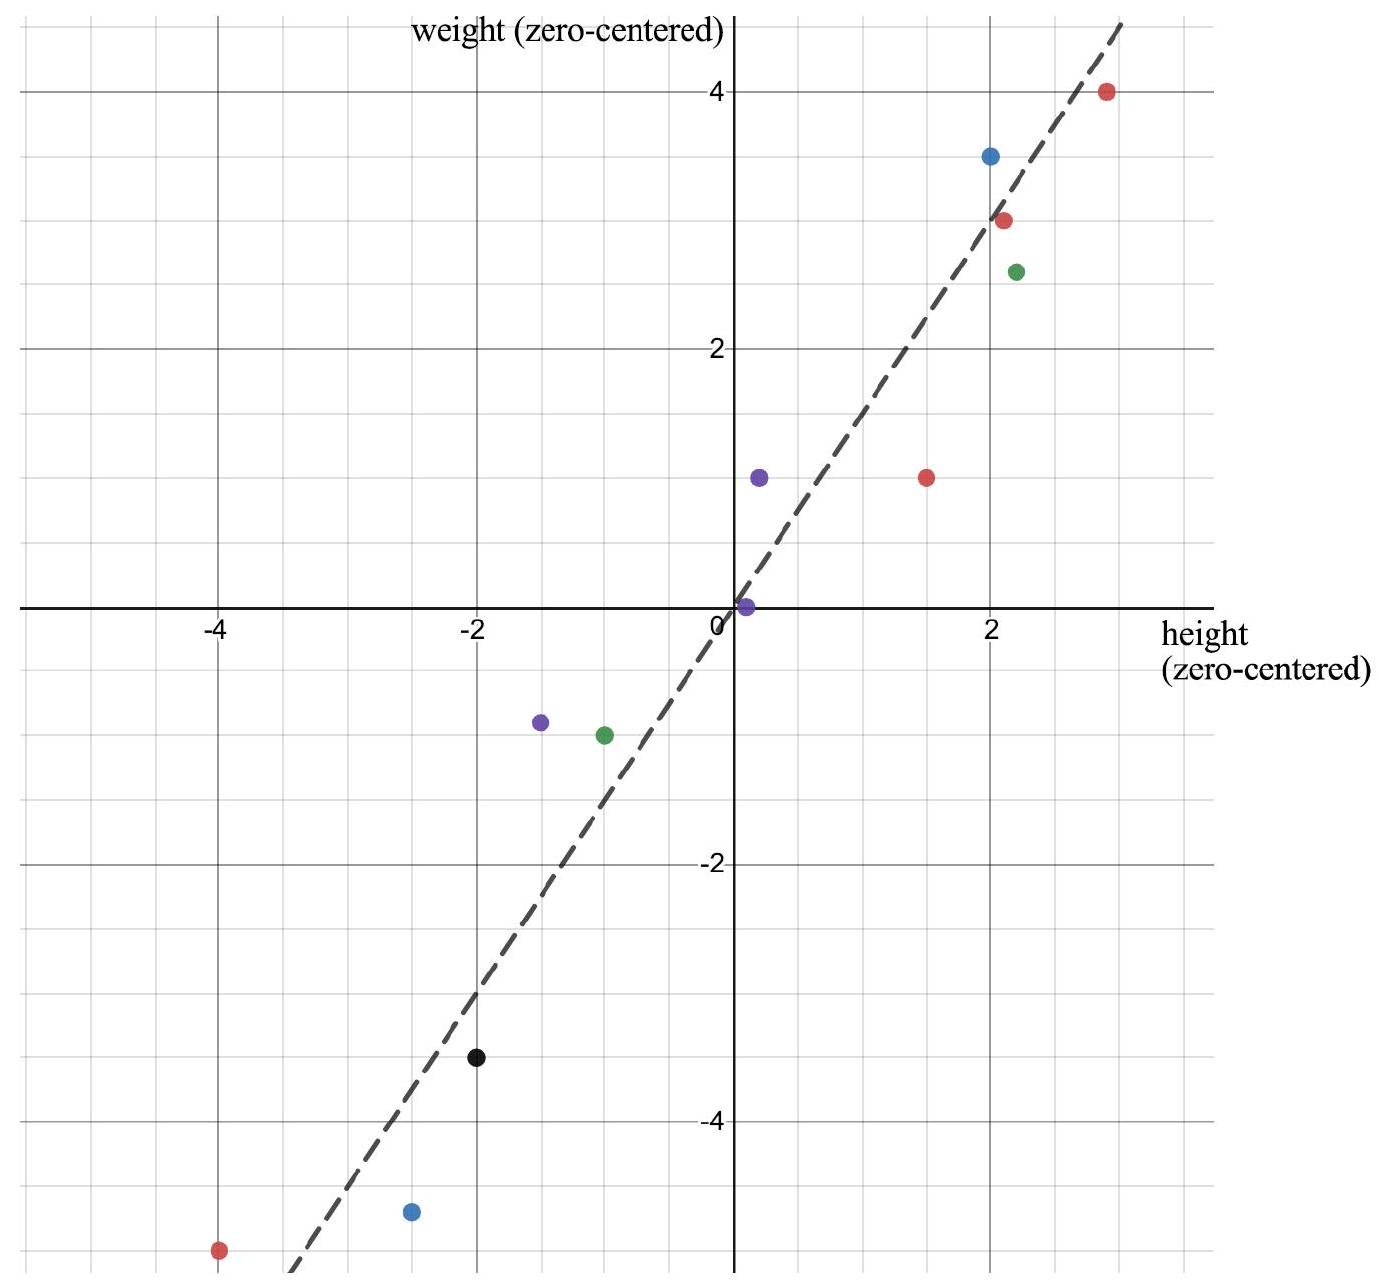
\includegraphics{images/day_14_fig1.jpg}

\begin{center}\rule{0.5\linewidth}{0.5pt}\end{center}

\subsection{\texorpdfstring{\emph{Plotting}}{Plotting}}\label{plotting}

\begin{verbatim}
<Figure size 1650x1050 with 0 Axes>
\end{verbatim}


\includegraphics{day_14_files/figure-pdf/cell-2-output-2.pdf}

\begin{center}\rule{0.5\linewidth}{0.5pt}\end{center}

\subsection{\texorpdfstring{\emph{The matrix \(U\): directions among
variables}}{The matrix U: directions among variables}}\label{the-matrix-u-directions-among-variables}

The columns of \(U\) live in \textbf{height--weight space}.

Each column \(u_i\) is a direction that can be drawn directly on the
scatterplot.

\begin{Shaded}
\begin{Highlighting}[]
\NormalTok{plt.clf()}

\NormalTok{plt.scatter(data.T[:,}\DecValTok{0}\NormalTok{], data.T[:,}\DecValTok{1}\NormalTok{], label}\OperatorTok{=}\StringTok{\textquotesingle{}Data\textquotesingle{}}\NormalTok{)}
\NormalTok{plt.quiver(}\DecValTok{0}\NormalTok{, }\DecValTok{0}\NormalTok{, Ud[}\DecValTok{0}\NormalTok{,}\DecValTok{0}\NormalTok{]}\OperatorTok{*}\NormalTok{Sd[}\DecValTok{0}\NormalTok{,}\DecValTok{0}\NormalTok{]}\OperatorTok{/}\DecValTok{5}\NormalTok{, Ud[}\DecValTok{1}\NormalTok{,}\DecValTok{0}\NormalTok{]}\OperatorTok{*}\NormalTok{Sd[}\DecValTok{0}\NormalTok{,}\DecValTok{0}\NormalTok{]}\OperatorTok{/}\DecValTok{5}\NormalTok{, angles}\OperatorTok{=}\StringTok{\textquotesingle{}xy\textquotesingle{}}\NormalTok{, scale\_units}\OperatorTok{=}\StringTok{\textquotesingle{}xy\textquotesingle{}}\NormalTok{, scale}\OperatorTok{=}\DecValTok{1}\NormalTok{, color}\OperatorTok{=}\StringTok{\textquotesingle{}red\textquotesingle{}}\NormalTok{, label}\OperatorTok{=}\VerbatimStringTok{r\textquotesingle{}$\textbackslash{}mathbf}\SpecialCharTok{\{u\}}\VerbatimStringTok{\_1$ ($\textbackslash{}sigma\_1$)\textquotesingle{}}\NormalTok{)}
\NormalTok{plt.quiver(}\DecValTok{0}\NormalTok{, }\DecValTok{0}\NormalTok{, Ud[}\DecValTok{0}\NormalTok{,}\DecValTok{1}\NormalTok{]}\OperatorTok{*}\NormalTok{Sd[}\DecValTok{1}\NormalTok{,}\DecValTok{1}\NormalTok{]}\OperatorTok{/}\DecValTok{5}\NormalTok{, Ud[}\DecValTok{1}\NormalTok{,}\DecValTok{1}\NormalTok{]}\OperatorTok{*}\NormalTok{Sd[}\DecValTok{1}\NormalTok{,}\DecValTok{1}\NormalTok{]}\OperatorTok{/}\DecValTok{5}\NormalTok{, angles}\OperatorTok{=}\StringTok{\textquotesingle{}xy\textquotesingle{}}\NormalTok{, scale\_units}\OperatorTok{=}\StringTok{\textquotesingle{}xy\textquotesingle{}}\NormalTok{, scale}\OperatorTok{=}\DecValTok{1}\NormalTok{, color}\OperatorTok{=}\StringTok{\textquotesingle{}blue\textquotesingle{}}\NormalTok{, label}\OperatorTok{=}\VerbatimStringTok{r\textquotesingle{}$\textbackslash{}mathbf}\SpecialCharTok{\{u\}}\VerbatimStringTok{\_2$ ($\textbackslash{}sigma\_2$)\textquotesingle{}}\NormalTok{)}
\NormalTok{plt.xlabel(}\StringTok{\textquotesingle{}Height\textquotesingle{}}\NormalTok{)}
\NormalTok{plt.ylabel(}\StringTok{\textquotesingle{}Weight\textquotesingle{}}\NormalTok{)}
\NormalTok{plt.axis(}\StringTok{\textquotesingle{}equal\textquotesingle{}}\NormalTok{)}
\NormalTok{plt.legend()}
\NormalTok{plt.show()}
\end{Highlighting}
\end{Shaded}


\includegraphics{day_14_files/figure-pdf/cell-3-output-1.pdf}

Each vector \(u_i\) answers:

\begin{quote}
\textbf{If the data vary according to one underlying pattern, how do the
measurements change?}
\end{quote}

\subsection{\texorpdfstring{\emph{}}{}}\label{section}

\begin{Shaded}
\begin{Highlighting}[]
\NormalTok{plt.clf()}

\NormalTok{plt.scatter(data.T[:,}\DecValTok{0}\NormalTok{], data.T[:,}\DecValTok{1}\NormalTok{], label}\OperatorTok{=}\StringTok{\textquotesingle{}Data\textquotesingle{}}\NormalTok{)}
\NormalTok{plt.quiver(}\DecValTok{0}\NormalTok{, }\DecValTok{0}\NormalTok{, Ud[}\DecValTok{0}\NormalTok{,}\DecValTok{0}\NormalTok{]}\OperatorTok{*}\NormalTok{Sd[}\DecValTok{0}\NormalTok{,}\DecValTok{0}\NormalTok{]}\OperatorTok{/}\DecValTok{5}\NormalTok{, Ud[}\DecValTok{1}\NormalTok{,}\DecValTok{0}\NormalTok{]}\OperatorTok{*}\NormalTok{Sd[}\DecValTok{0}\NormalTok{,}\DecValTok{0}\NormalTok{]}\OperatorTok{/}\DecValTok{5}\NormalTok{, angles}\OperatorTok{=}\StringTok{\textquotesingle{}xy\textquotesingle{}}\NormalTok{, scale\_units}\OperatorTok{=}\StringTok{\textquotesingle{}xy\textquotesingle{}}\NormalTok{, scale}\OperatorTok{=}\DecValTok{1}\NormalTok{, color}\OperatorTok{=}\StringTok{\textquotesingle{}red\textquotesingle{}}\NormalTok{, label}\OperatorTok{=}\VerbatimStringTok{r\textquotesingle{}$\textbackslash{}mathbf}\SpecialCharTok{\{u\}}\VerbatimStringTok{\_1$ ($\textbackslash{}sigma\_1$)\textquotesingle{}}\NormalTok{)}
\NormalTok{plt.quiver(}\DecValTok{0}\NormalTok{, }\DecValTok{0}\NormalTok{, Ud[}\DecValTok{0}\NormalTok{,}\DecValTok{1}\NormalTok{]}\OperatorTok{*}\NormalTok{Sd[}\DecValTok{1}\NormalTok{,}\DecValTok{1}\NormalTok{]}\OperatorTok{/}\DecValTok{5}\NormalTok{, Ud[}\DecValTok{1}\NormalTok{,}\DecValTok{1}\NormalTok{]}\OperatorTok{*}\NormalTok{Sd[}\DecValTok{1}\NormalTok{,}\DecValTok{1}\NormalTok{]}\OperatorTok{/}\DecValTok{5}\NormalTok{, angles}\OperatorTok{=}\StringTok{\textquotesingle{}xy\textquotesingle{}}\NormalTok{, scale\_units}\OperatorTok{=}\StringTok{\textquotesingle{}xy\textquotesingle{}}\NormalTok{, scale}\OperatorTok{=}\DecValTok{1}\NormalTok{, color}\OperatorTok{=}\StringTok{\textquotesingle{}blue\textquotesingle{}}\NormalTok{, label}\OperatorTok{=}\VerbatimStringTok{r\textquotesingle{}$\textbackslash{}mathbf}\SpecialCharTok{\{u\}}\VerbatimStringTok{\_2$ ($\textbackslash{}sigma\_2$)\textquotesingle{}}\NormalTok{)}
\NormalTok{plt.xlabel(}\StringTok{\textquotesingle{}Height\textquotesingle{}}\NormalTok{)}
\NormalTok{plt.ylabel(}\StringTok{\textquotesingle{}Weight\textquotesingle{}}\NormalTok{)}
\NormalTok{plt.axis(}\StringTok{\textquotesingle{}equal\textquotesingle{}}\NormalTok{)}
\NormalTok{plt.legend()}
\NormalTok{plt.show()}
\end{Highlighting}
\end{Shaded}


\includegraphics{day_14_files/figure-pdf/cell-4-output-1.pdf}

Typical interpretation:

\begin{itemize}
\item
  \(u_1\): height and weight increase together → overall \textbf{body
  size} direction.
\item
  \(u_2\): height increases while weight decreases (or vice versa) →
  \textbf{body proportion} differences.
\end{itemize}

So \(U\) provides an orthogonal coordinate system describing \textbf{how
measurements change}.

\begin{center}\rule{0.5\linewidth}{0.5pt}\end{center}

\subsection{\texorpdfstring{\emph{The matrix \(V\): patterns among
people}}{The matrix V: patterns among people}}\label{the-matrix-v-patterns-among-people}

The matrix \(V\) lives in \textbf{person space}.

Each column \(v_i\) assigns a number to every person.

\begin{Shaded}
\begin{Highlighting}[]
\NormalTok{plt.clf()}
\NormalTok{plt.imshow(Vd.T[:}\DecValTok{2}\NormalTok{,:])}
\NormalTok{plt.show()}
\end{Highlighting}
\end{Shaded}


\includegraphics{day_14_files/figure-pdf/cell-5-output-1.pdf}

Each vector \(v_i\) tells us:

\begin{quote}
\textbf{which people participate in a particular pattern of variation.}
\end{quote}

Interpretation:

\begin{itemize}
\tightlist
\item
  Large positive entry → that person strongly follows the pattern.
\item
  Negative entry → participates in the opposite way.
\item
  Near zero → little involvement.
\end{itemize}

Examples:

\begin{itemize}
\tightlist
\item
  The first pattern (in the first row) separates larger vs.~smaller
  individuals.
\item
  The second pattern (in the second row) contrasts tall--light
  vs.~short--heavy people.
\end{itemize}

Because measurements live in a 2-dimensional space (height and weight),
only \textbf{two independent population patterns} are needed.

\begin{center}\rule{0.5\linewidth}{0.5pt}\end{center}

\subsection{\texorpdfstring{\emph{Reconstructing the
data}}{Reconstructing the data}}\label{reconstructing-the-data}

Using the first two rows of \(V^T\), scaled by the singular values and
rotated by \(U\):

\begin{Shaded}
\begin{Highlighting}[]
\NormalTok{plt.clf()}
\NormalTok{component1 }\OperatorTok{=}\NormalTok{ np.outer(Vd.T[:,}\DecValTok{0}\NormalTok{],Sd[}\DecValTok{0}\NormalTok{,}\DecValTok{0}\NormalTok{]}\OperatorTok{*}\NormalTok{Ud[}\DecValTok{0}\NormalTok{])}
\NormalTok{component2 }\OperatorTok{=}\NormalTok{ np.outer(Vd.T[:,}\DecValTok{1}\NormalTok{],Sd[}\DecValTok{1}\NormalTok{,}\DecValTok{1}\NormalTok{]}\OperatorTok{*}\NormalTok{Ud[}\DecValTok{1}\NormalTok{])}
\NormalTok{plt.scatter(component1[:,}\DecValTok{0}\NormalTok{],component1[:,}\DecValTok{1}\NormalTok{])}
\NormalTok{plt.scatter(component2[:,}\DecValTok{0}\NormalTok{],component2[:,}\DecValTok{1}\NormalTok{])}
\NormalTok{combined }\OperatorTok{=}\NormalTok{ component1 }\OperatorTok{+}\NormalTok{ component2}
\NormalTok{plt.scatter(combined[:,}\DecValTok{0}\NormalTok{],combined[:,}\DecValTok{1}\NormalTok{])}
\NormalTok{plt.axis(}\StringTok{\textquotesingle{}equal\textquotesingle{}}\NormalTok{)}
\NormalTok{plt.legend([}\StringTok{"component 1"}\NormalTok{, }\StringTok{"component 2"}\NormalTok{, }\StringTok{"component 1 + component 2"}\NormalTok{])}
\NormalTok{plt.show()}
\end{Highlighting}
\end{Shaded}


\includegraphics{day_14_files/figure-pdf/cell-6-output-1.pdf}

Each term of the SVD

\[
A = U S V^\mathsf{T}
\]

can be written as

\[
A
=
\sigma_1 u_1 v_1^\mathsf{T}
+
\dots
+
\sigma_r u_r v_r^\mathsf{T}.
\]

Each component means:

\begin{itemize}
\tightlist
\item
  \(v_i\): how much this individual participates in the pattern,
\item
  \(u_i\): how height and weight change,
\item
  \(\sigma_i\): how important this pattern is.
\end{itemize}

\begin{center}\rule{0.5\linewidth}{0.5pt}\end{center}

\subsection{\texorpdfstring{\emph{Skills}}{Skills}}\label{skills}

\begin{itemize}
\item
  Interpret the columns of \(U\) as directions of change in measurement
  space.
\item
  Interpret the columns of \(V\) as independent patterns among
  individuals.
\item
  Express the matrix as a sum of outer products
  \(\sigma_i \mathbf{u}_i \mathbf{v}_i^T\). lls
\item
  Interpret the columns of \(U\) as capturing relationships between rows
  of the data matrix
\item
  Interpret the rows of \(V^T\) as capturing relationships between
  columns
\item
  Express the matrix as a sum of outer products
  \(\sigma_i \mathbf{u}_i \mathbf{v}_i^T\)
\end{itemize}

\section{\texorpdfstring{\emph{SVD on
images}}{SVD on images}}\label{svd-on-images}

SVD for image compression; left/right singular vectors; color images;
PCA as truncated SVD.

\subsection{\texorpdfstring{\emph{Motivation: a
cat}}{Motivation: a cat}}\label{motivation-a-cat}

\begin{Shaded}
\begin{Highlighting}[]
\CommentTok{\# display the path of the current python environment}

\ImportTok{import}\NormalTok{ cv2}

\NormalTok{image }\OperatorTok{=}\NormalTok{ cv2.imread(}\StringTok{\textquotesingle{}test\_cat.png\textquotesingle{}}\NormalTok{, cv2.IMREAD\_GRAYSCALE)}
\NormalTok{plt.figure(figsize}\OperatorTok{=}\NormalTok{(}\DecValTok{2}\NormalTok{, }\DecValTok{2}\NormalTok{))}
\NormalTok{plt.imshow(image, cmap}\OperatorTok{=}\StringTok{\textquotesingle{}gray\textquotesingle{}}\NormalTok{)}
\NormalTok{plt.title(}\StringTok{\textquotesingle{}Cat Image\textquotesingle{}}\NormalTok{)}
\NormalTok{plt.show()}
\end{Highlighting}
\end{Shaded}


\includegraphics{day_14_files/figure-pdf/cell-7-output-1.pdf}

\subsection{\texorpdfstring{\emph{Dimensions of the
decomposition}}{Dimensions of the decomposition}}\label{dimensions-of-the-decomposition}

What are the dimensions of the decompositions for an image?

\begin{Shaded}
\begin{Highlighting}[]
\NormalTok{U, S, Vt }\OperatorTok{=}\NormalTok{ np.linalg.svd(image, full\_matrices}\OperatorTok{=}\VariableTok{False}\NormalTok{)}
\BuiltInTok{print}\NormalTok{(}\SpecialStringTok{f\textquotesingle{}The shape of U is }\SpecialCharTok{\{}\NormalTok{U}\SpecialCharTok{.}\NormalTok{shape}\SpecialCharTok{\}}\SpecialStringTok{, the shape of S is }\SpecialCharTok{\{}\NormalTok{S}\SpecialCharTok{.}\NormalTok{shape}\SpecialCharTok{\}}\SpecialStringTok{, the shape of V is }\SpecialCharTok{\{}\NormalTok{Vt}\SpecialCharTok{.}\NormalTok{shape}\SpecialCharTok{\}}\SpecialStringTok{\textquotesingle{}}\NormalTok{)}
\end{Highlighting}
\end{Shaded}

\begin{verbatim}
The shape of U is (360, 360), the shape of S is (360,), the shape of V is (360, 360)
\end{verbatim}

. . .

\textbf{Left singular values}, corresponding to U, are the eigenvalues
of \(AA^T\). For an image, \(AA^T\) is the covariance matrix of the rows
of \(A\).

. . .

\textbf{Right singular values} are the eigenvalues of \(A^{T}A\). For an
image, \(A^TA\) is the covariance matrix of the columns of \(A\).

\subsection{\texorpdfstring{\emph{Simple
example}}{Simple example}}\label{simple-example}

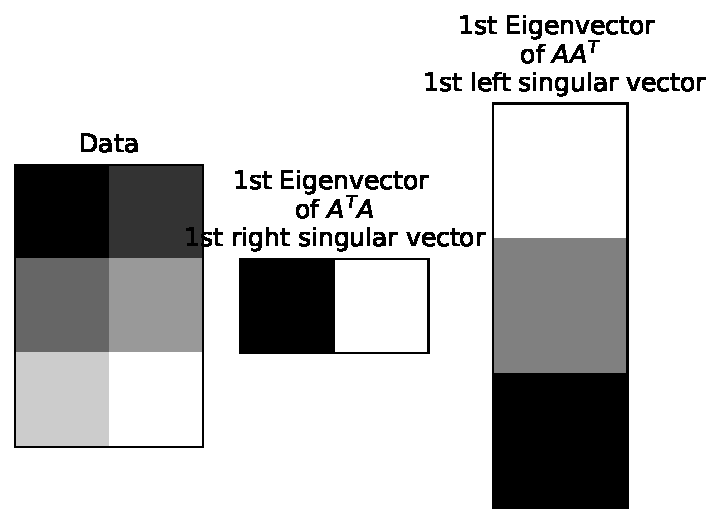
\includegraphics{day_14_files/figure-pdf/cell-9-output-1.pdf}

\subsection{\texorpdfstring{\emph{Reconstructing our
matrix}}{Reconstructing our matrix}}\label{reconstructing-our-matrix}

\begin{Shaded}
\begin{Highlighting}[]
\NormalTok{U, S, Vt }\OperatorTok{=}\NormalTok{ np.linalg.svd(A, full\_matrices}\OperatorTok{=}\VariableTok{False}\NormalTok{)}
\NormalTok{ax1 }\OperatorTok{=}\NormalTok{ plt.subplot(}\DecValTok{141}\NormalTok{)}
\NormalTok{ax2 }\OperatorTok{=}\NormalTok{ plt.subplot(}\DecValTok{142}\NormalTok{)}
\NormalTok{ax3 }\OperatorTok{=}\NormalTok{ plt.subplot(}\DecValTok{143}\NormalTok{)}
\NormalTok{ax4 }\OperatorTok{=}\NormalTok{ plt.subplot(}\DecValTok{144}\NormalTok{)}
\NormalTok{ax1.imshow(A, cmap}\OperatorTok{=}\StringTok{\textquotesingle{}gray\textquotesingle{}}\NormalTok{)}
\NormalTok{ax2.imshow(np.outer(U[:,}\DecValTok{0}\NormalTok{], Vt[}\DecValTok{0}\NormalTok{,:])}\OperatorTok{*}\NormalTok{S[}\DecValTok{0}\NormalTok{], cmap}\OperatorTok{=}\StringTok{\textquotesingle{}gray\textquotesingle{}}\NormalTok{)}
\NormalTok{ax3.imshow(np.outer(U[:,}\DecValTok{1}\NormalTok{], Vt[}\DecValTok{1}\NormalTok{,:])}\OperatorTok{*}\NormalTok{S[}\DecValTok{1}\NormalTok{], cmap}\OperatorTok{=}\StringTok{\textquotesingle{}gray\textquotesingle{}}\NormalTok{)}
\NormalTok{ax4.imshow(np.outer(U[:,}\DecValTok{0}\NormalTok{], Vt[}\DecValTok{0}\NormalTok{,:])}\OperatorTok{*}\NormalTok{S[}\DecValTok{0}\NormalTok{]}\OperatorTok{+}\NormalTok{np.outer(U[:,}\DecValTok{1}\NormalTok{], Vt[}\DecValTok{1}\NormalTok{,:])}\OperatorTok{*}\NormalTok{S[}\DecValTok{1}\NormalTok{], cmap}\OperatorTok{=}\StringTok{\textquotesingle{}gray\textquotesingle{}}\NormalTok{)}
\ControlFlowTok{for}\NormalTok{ ax }\KeywordTok{in}\NormalTok{ [ax1, ax2, ax3,ax4]:}
\NormalTok{  ax.axes.xaxis.set\_ticks([])}
\NormalTok{  ax.axes.yaxis.set\_ticks([])}
\NormalTok{ax1.set\_title(}\StringTok{\textquotesingle{}Data\textquotesingle{}}\NormalTok{)}
\NormalTok{ax2.set\_title(}\StringTok{\textquotesingle{}1st component }\CharTok{\textbackslash{}n}\StringTok{ * $\textbackslash{}sigma\_1$\textquotesingle{}}\NormalTok{)}
\NormalTok{ax3.set\_title(}\StringTok{\textquotesingle{}2nd component }\CharTok{\textbackslash{}n}\StringTok{ * $\textbackslash{}sigma\_2$\textquotesingle{}}\NormalTok{)}
\NormalTok{ax4.set\_title(}\StringTok{\textquotesingle{}1st + 2nd }\CharTok{\textbackslash{}n}\StringTok{ component\textquotesingle{}}\NormalTok{)}
\NormalTok{plt.show()}
\end{Highlighting}
\end{Shaded}


\includegraphics{day_14_files/figure-pdf/cell-10-output-1.pdf}

How much of the variance is captured by the first two components?

The variance captured by each component is the sum of the squares of the
singular values divided by the sum of the squares of all the singular
values.

\subsection{\texorpdfstring{\emph{Back to the
cat}}{Back to the cat}}\label{back-to-the-cat}

\begin{Shaded}
\begin{Highlighting}[]
\CommentTok{\# !pip3 install opencv{-}python}

\NormalTok{plt.imshow(image, cmap}\OperatorTok{=}\StringTok{\textquotesingle{}gray\textquotesingle{}}\NormalTok{)}
\NormalTok{plt.title(}\StringTok{\textquotesingle{}Cat Image\textquotesingle{}}\NormalTok{)}
\NormalTok{plt.show()}
\end{Highlighting}
\end{Shaded}


\includegraphics{day_14_files/figure-pdf/cell-11-output-1.pdf}

\begin{Shaded}
\begin{Highlighting}[]
\NormalTok{U, S, Vt }\OperatorTok{=}\NormalTok{ np.linalg.svd(image, full\_matrices}\OperatorTok{=}\VariableTok{False}\NormalTok{)}
\end{Highlighting}
\end{Shaded}

\begin{Shaded}
\begin{Highlighting}[]
\NormalTok{fig }\OperatorTok{=}\NormalTok{ plt.figure(figsize}\OperatorTok{=}\NormalTok{(}\DecValTok{12}\NormalTok{, }\DecValTok{6}\NormalTok{))}
\NormalTok{imsub }\OperatorTok{=}\NormalTok{ image}\OperatorTok{{-}}\NormalTok{np.mean(image,axis}\OperatorTok{=}\DecValTok{0}\NormalTok{)}
\NormalTok{imsub }\OperatorTok{=}\NormalTok{ imsub }\OperatorTok{{-}}\NormalTok{ np.mean(imsub,axis}\OperatorTok{=}\DecValTok{1}\NormalTok{)}
\NormalTok{aat}\OperatorTok{=}\NormalTok{imsub}\OperatorTok{@}\NormalTok{imsub.T}
\NormalTok{ata}\OperatorTok{=}\NormalTok{imsub.T}\OperatorTok{@}\NormalTok{imsub}
\NormalTok{ax1}\OperatorTok{=}\NormalTok{fig.add\_subplot(}\DecValTok{121}\NormalTok{)}
\NormalTok{ax1.imshow(ata)}


\NormalTok{ax2}\OperatorTok{=}\NormalTok{fig.add\_subplot(}\DecValTok{122}\NormalTok{)}
\NormalTok{ax2.imshow(aat)}
\NormalTok{ax2.set\_title(}\StringTok{"AA\^{}T"}\NormalTok{)}
\NormalTok{ax1.set\_title(}\StringTok{"A\^{}TA"}\NormalTok{)}
\NormalTok{plt.show()}
\end{Highlighting}
\end{Shaded}

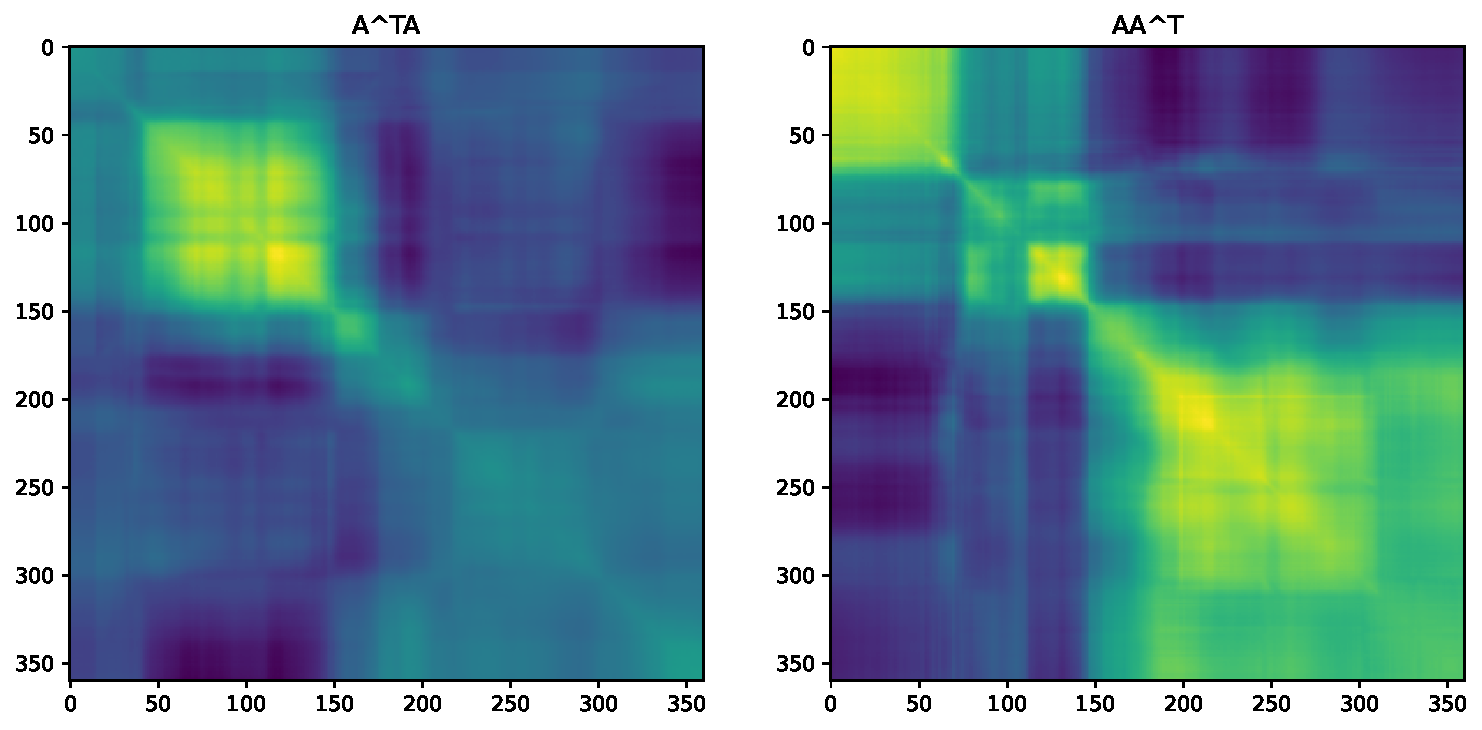
\includegraphics{day_14_files/figure-pdf/cell-13-output-1.pdf}

\subsection{\texorpdfstring{\emph{First Singular
Value}}{First Singular Value}}\label{first-singular-value}

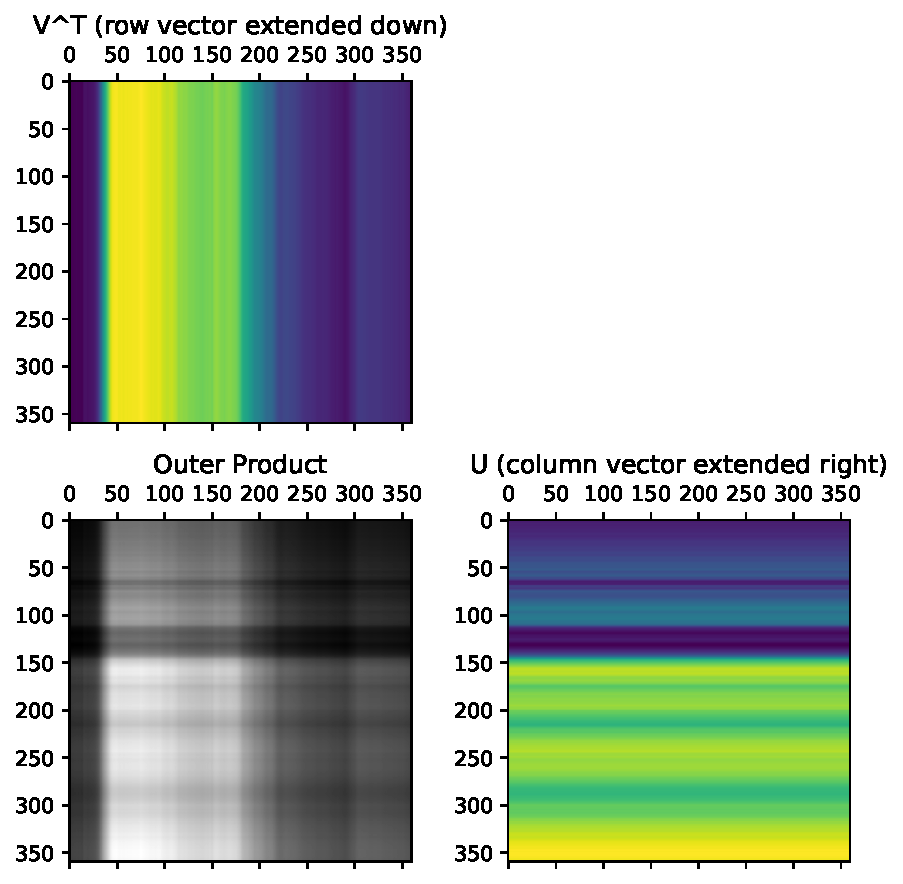
\includegraphics{day_14_files/figure-pdf/cell-14-output-1.pdf}

\subsection{\texorpdfstring{\emph{Second Singular
Value}}{Second Singular Value}}\label{second-singular-value}

\begin{Shaded}
\begin{Highlighting}[]
\NormalTok{plot\_uv(}\DecValTok{1}\NormalTok{)}
\end{Highlighting}
\end{Shaded}

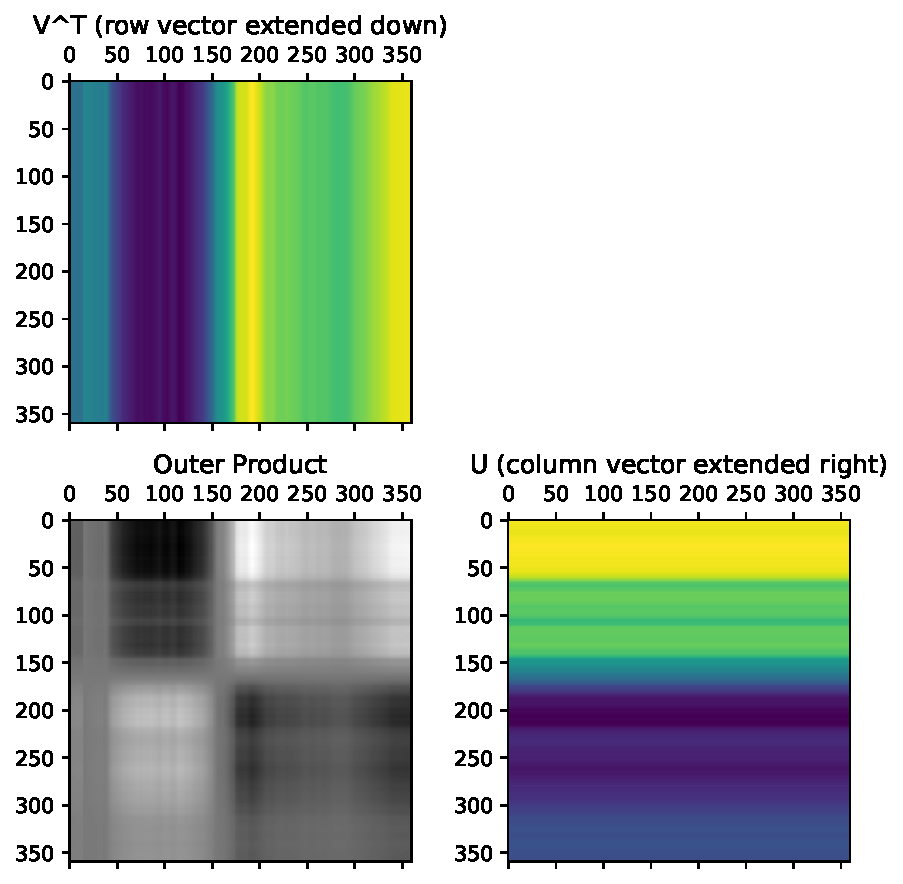
\includegraphics{day_14_files/figure-pdf/cell-15-output-1.pdf}

\subsection{\texorpdfstring{\emph{Third Singular
Value}}{Third Singular Value}}\label{third-singular-value}

\begin{Shaded}
\begin{Highlighting}[]
\NormalTok{plot\_uv(}\DecValTok{2}\NormalTok{)}
\end{Highlighting}
\end{Shaded}

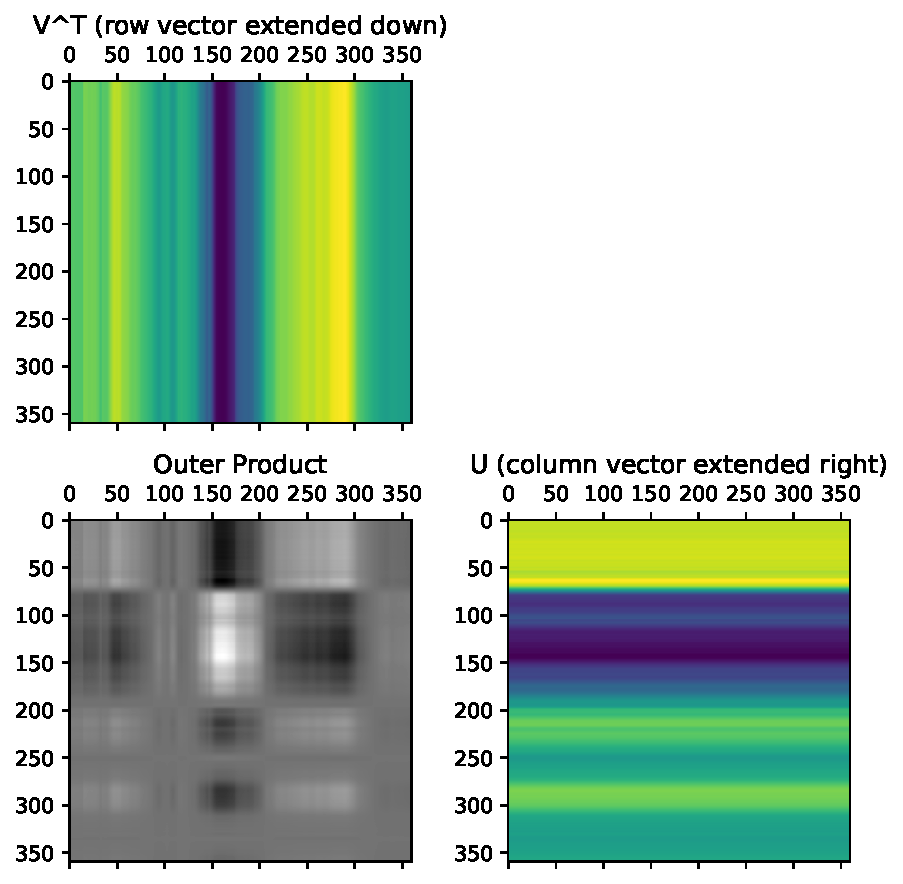
\includegraphics{day_14_files/figure-pdf/cell-16-output-1.pdf}

\subsection{\texorpdfstring{\emph{Adding them
up}}{Adding them up}}\label{adding-them-up}

\begin{Shaded}
\begin{Highlighting}[]
\NormalTok{fig }\OperatorTok{=}\NormalTok{ plt.figure(figsize}\OperatorTok{=}\NormalTok{(}\DecValTok{12}\NormalTok{, }\DecValTok{6}\NormalTok{))}
\ControlFlowTok{for}\NormalTok{ i }\KeywordTok{in} \BuiltInTok{range}\NormalTok{(}\DecValTok{3}\NormalTok{):}
\NormalTok{    reconstructed\_image }\OperatorTok{=}\NormalTok{ np.matrix(U[:,i:i}\OperatorTok{+}\DecValTok{1}\NormalTok{]) }\OperatorTok{*}\NormalTok{ np.diag(S[i:i}\OperatorTok{+}\DecValTok{1}\NormalTok{]) }\OperatorTok{*}\NormalTok{ np.matrix(Vt[i:i}\OperatorTok{+}\DecValTok{1}\NormalTok{,:])}
\NormalTok{    ax1 }\OperatorTok{=}\NormalTok{ fig.add\_subplot(}\DecValTok{131}\OperatorTok{+}\NormalTok{i)}
\NormalTok{    ax1.imshow(reconstructed\_image, cmap}\OperatorTok{=}\StringTok{\textquotesingle{}gray\textquotesingle{}}\NormalTok{)}
\NormalTok{    ax1.set\_title(}\SpecialStringTok{f\textquotesingle{}Image from Singular Value }\SpecialCharTok{\{}\NormalTok{i}\OperatorTok{+}\DecValTok{1}\SpecialCharTok{\}}\SpecialStringTok{\textquotesingle{}}\NormalTok{)}
\NormalTok{plt.show()}
\end{Highlighting}
\end{Shaded}

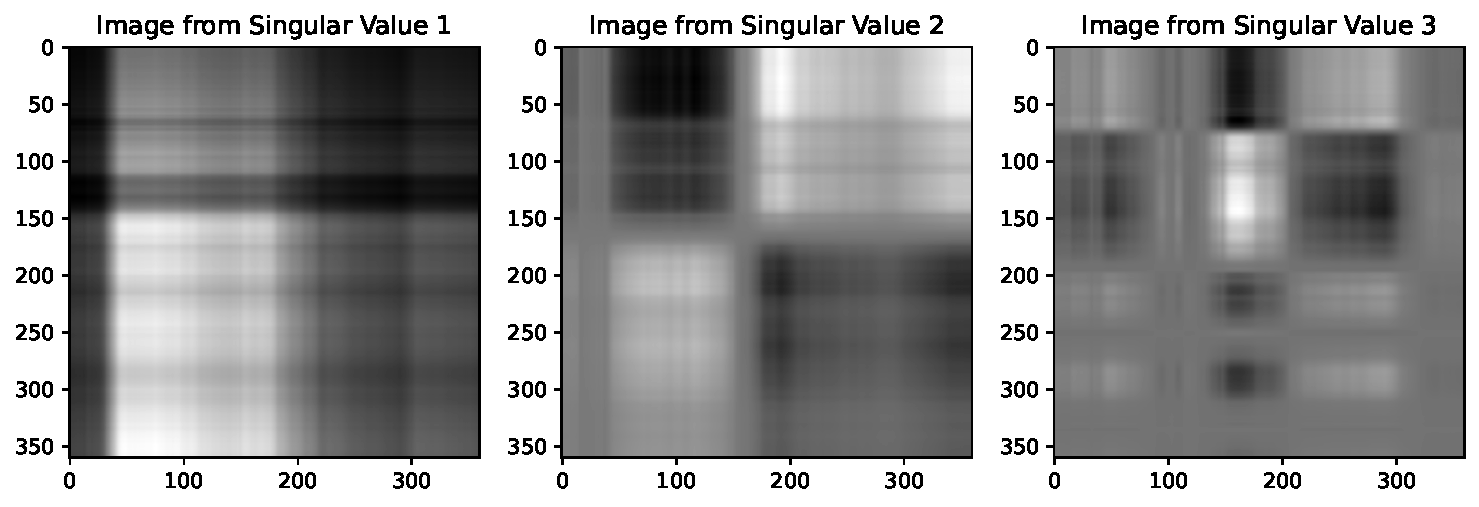
\includegraphics{day_14_files/figure-pdf/cell-17-output-1.pdf}

. . .

\begin{Shaded}
\begin{Highlighting}[]
\NormalTok{plt.figure(figsize}\OperatorTok{=}\NormalTok{(}\DecValTok{16}\NormalTok{,}\DecValTok{4}\NormalTok{))}

\CommentTok{\# start, end, step = 5, 25, 5}
\NormalTok{start, end, step }\OperatorTok{=} \DecValTok{1}\NormalTok{, }\DecValTok{5}\NormalTok{, }\DecValTok{1}
\ControlFlowTok{for}\NormalTok{ i }\KeywordTok{in} \BuiltInTok{range}\NormalTok{(start, end, step):}
\NormalTok{    plt.subplot(}\DecValTok{1}\NormalTok{, (end }\OperatorTok{{-}}\NormalTok{ start) }\OperatorTok{//}\NormalTok{ step }\OperatorTok{+} \DecValTok{1}\NormalTok{, (i }\OperatorTok{{-}}\NormalTok{ start) }\OperatorTok{//}\NormalTok{ step }\OperatorTok{+} \DecValTok{1}\NormalTok{)}
\NormalTok{    reconstructed }\OperatorTok{=}\NormalTok{ np.matrix(U[:, :i]) }\OperatorTok{*}\NormalTok{ np.diag(S[:i]) }\OperatorTok{*}\NormalTok{ np.matrix(Vt[:i, :])}
\NormalTok{    plt.imshow(reconstructed, cmap}\OperatorTok{=}\StringTok{\textquotesingle{}gray\textquotesingle{}}\NormalTok{)}
\NormalTok{    plt.title(}\StringTok{\textquotesingle{}n = }\SpecialCharTok{\%s}\StringTok{\textquotesingle{}} \OperatorTok{\%}\NormalTok{ i)}

\NormalTok{plt.tight\_layout()}
\NormalTok{plt.show()}
\end{Highlighting}
\end{Shaded}

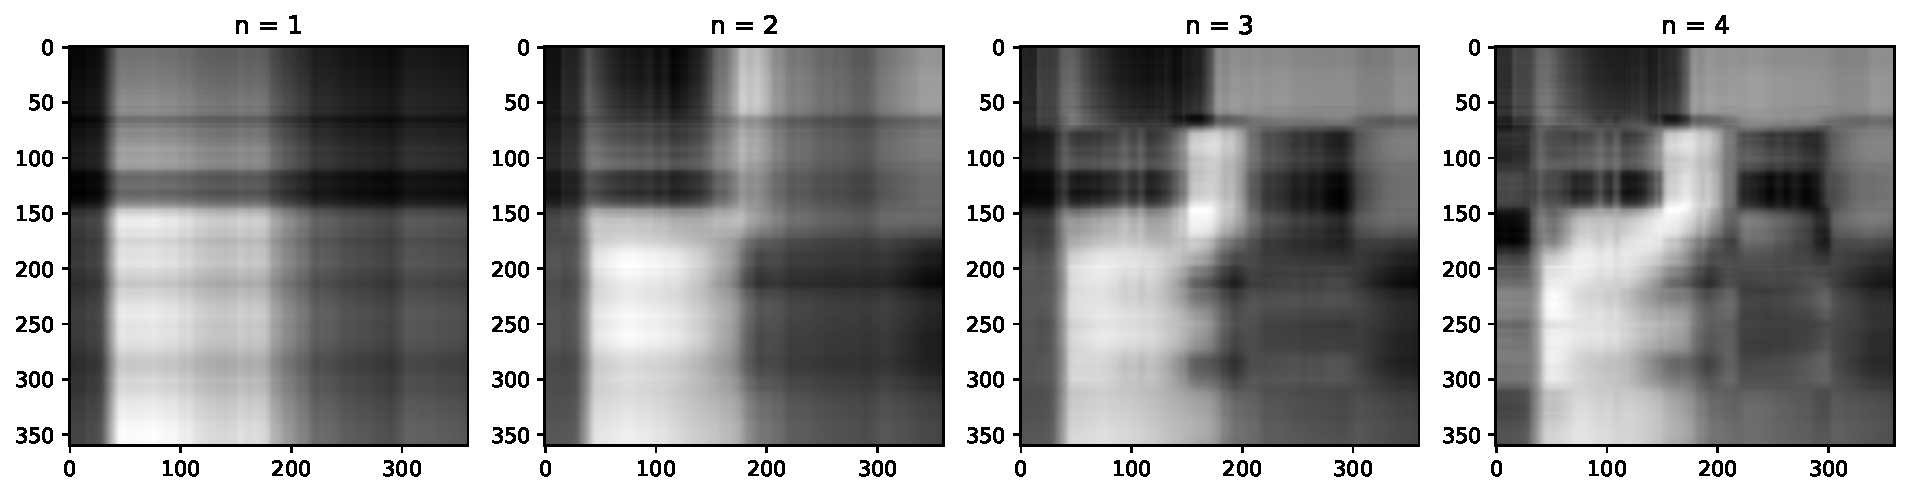
\includegraphics{day_14_files/figure-pdf/cell-18-output-1.pdf}

\subsection{\texorpdfstring{\emph{}}{}}\label{section-1}

\begin{Shaded}
\begin{Highlighting}[]
\NormalTok{plt.figure(figsize}\OperatorTok{=}\NormalTok{(}\DecValTok{16}\NormalTok{,}\DecValTok{4}\NormalTok{))}

\NormalTok{start, end, step }\OperatorTok{=} \DecValTok{5}\NormalTok{, }\DecValTok{25}\NormalTok{, }\DecValTok{5}
\CommentTok{\#start, end, step = 1, 5, 1}
\ControlFlowTok{for}\NormalTok{ i }\KeywordTok{in} \BuiltInTok{range}\NormalTok{(start, end, step):}
\NormalTok{    plt.subplot(}\DecValTok{1}\NormalTok{, (end }\OperatorTok{{-}}\NormalTok{ start) }\OperatorTok{//}\NormalTok{ step }\OperatorTok{+} \DecValTok{1}\NormalTok{, (i }\OperatorTok{{-}}\NormalTok{ start) }\OperatorTok{//}\NormalTok{ step }\OperatorTok{+} \DecValTok{1}\NormalTok{)}
\NormalTok{    reconstructed }\OperatorTok{=}\NormalTok{ np.matrix(U[:, :i]) }\OperatorTok{*}\NormalTok{ np.diag(S[:i]) }\OperatorTok{*}\NormalTok{ np.matrix(Vt[:i, :])}
\NormalTok{    plt.imshow(reconstructed, cmap}\OperatorTok{=}\StringTok{\textquotesingle{}gray\textquotesingle{}}\NormalTok{)}
\NormalTok{    plt.title(}\StringTok{\textquotesingle{}n = }\SpecialCharTok{\%s}\StringTok{\textquotesingle{}} \OperatorTok{\%}\NormalTok{ i)}

\NormalTok{plt.tight\_layout()}
\NormalTok{plt.show()}
\end{Highlighting}
\end{Shaded}

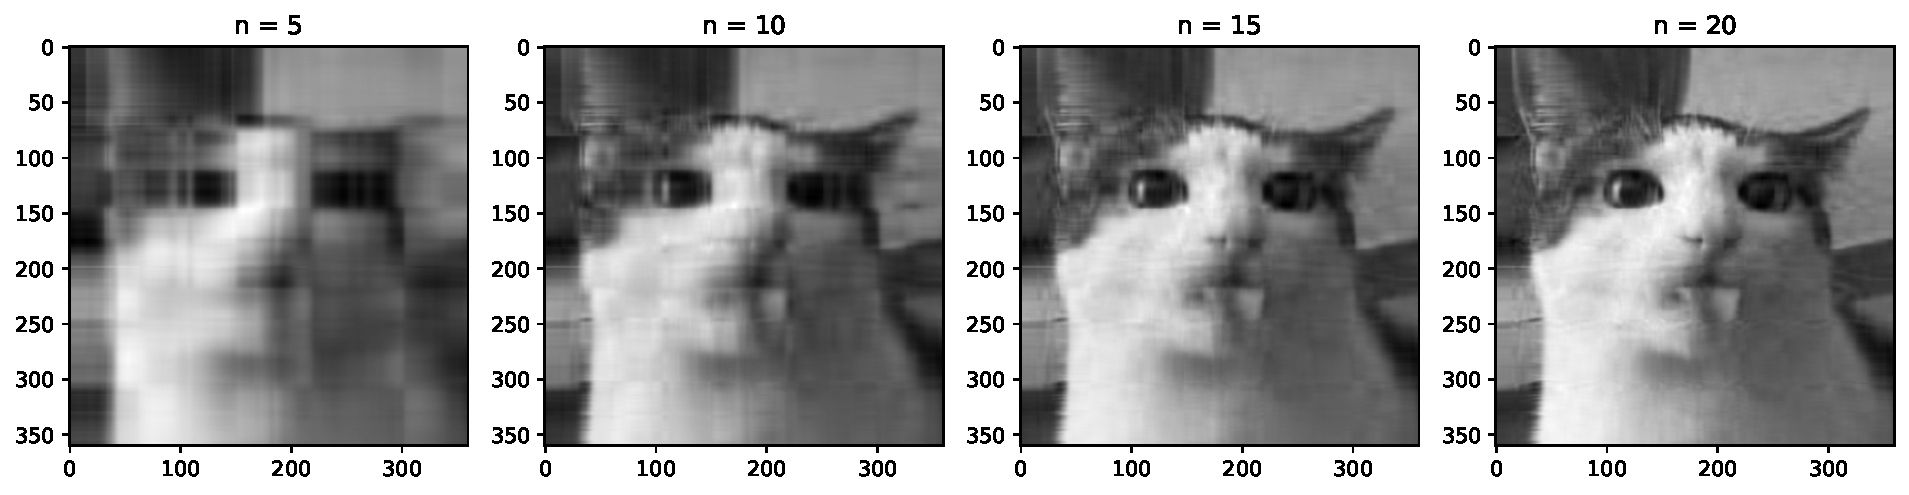
\includegraphics{day_14_files/figure-pdf/cell-19-output-1.pdf}

\subsection{\texorpdfstring{\emph{Color
images}}{Color images}}\label{color-images}

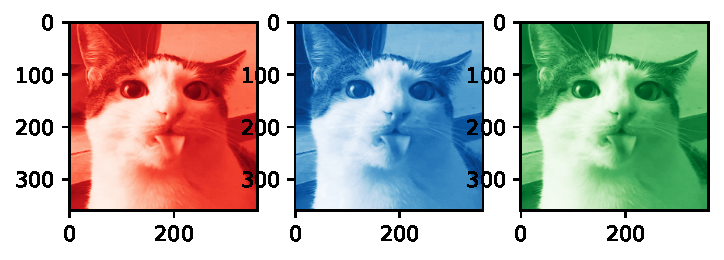
\includegraphics{day_14_files/figure-pdf/cell-20-output-1.pdf}

\begin{Shaded}
\begin{Highlighting}[]
\CommentTok{\# SVD for each channel}
\NormalTok{U\_R, S\_R, Vt\_R }\OperatorTok{=}\NormalTok{ np.linalg.svd(R, full\_matrices}\OperatorTok{=}\VariableTok{False}\NormalTok{)}
\NormalTok{U\_G, S\_G, Vt\_G }\OperatorTok{=}\NormalTok{ np.linalg.svd(G, full\_matrices}\OperatorTok{=}\VariableTok{False}\NormalTok{)}
\NormalTok{U\_B, S\_B, Vt\_B }\OperatorTok{=}\NormalTok{ np.linalg.svd(B, full\_matrices}\OperatorTok{=}\VariableTok{False}\NormalTok{)}

\NormalTok{n }\OperatorTok{=} \DecValTok{50}  \CommentTok{\# rank approximation parameter}
\NormalTok{R\_compressed }\OperatorTok{=}\NormalTok{ np.matrix(U\_R[:, :n]) }\OperatorTok{*}\NormalTok{ np.diag(S\_R[:n]) }\OperatorTok{*}\NormalTok{ np.matrix(Vt\_R[:n, :])}
\NormalTok{G\_compressed }\OperatorTok{=}\NormalTok{ np.matrix(U\_G[:, :n]) }\OperatorTok{*}\NormalTok{ np.diag(S\_G[:n]) }\OperatorTok{*}\NormalTok{ np.matrix(Vt\_G[:n, :])}
\NormalTok{B\_compressed }\OperatorTok{=}\NormalTok{ np.matrix(U\_B[:, :n]) }\OperatorTok{*}\NormalTok{ np.diag(S\_B[:n]) }\OperatorTok{*}\NormalTok{ np.matrix(Vt\_B[:n, :])}

\CommentTok{\# Combining the compressed channels}
\NormalTok{compressed\_image }\OperatorTok{=}\NormalTok{ cv2.merge([np.clip(R\_compressed, }\DecValTok{1}\NormalTok{, }\DecValTok{255}\NormalTok{), np.clip(G\_compressed, }\DecValTok{1}\NormalTok{, }\DecValTok{255}\NormalTok{), np.clip(B\_compressed, }\DecValTok{1}\NormalTok{, }\DecValTok{255}\NormalTok{)])}
\NormalTok{compressed\_image }\OperatorTok{=}\NormalTok{ compressed\_image.astype(np.uint8)}
\NormalTok{plt.imshow(compressed\_image)}
\NormalTok{plt.title(}\StringTok{\textquotesingle{}n = }\SpecialCharTok{\%s}\StringTok{\textquotesingle{}} \OperatorTok{\%}\NormalTok{ n)}
\NormalTok{plt.show()}

\CommentTok{\# Plotting the compressed RGB channels}
\NormalTok{plt.subplot(}\DecValTok{1}\NormalTok{, }\DecValTok{3}\NormalTok{, }\DecValTok{1}\NormalTok{)}
\NormalTok{plt.imshow(R\_compressed, cmap}\OperatorTok{=}\StringTok{\textquotesingle{}Reds\_r\textquotesingle{}}\NormalTok{)}
\NormalTok{plt.subplot(}\DecValTok{1}\NormalTok{, }\DecValTok{3}\NormalTok{, }\DecValTok{2}\NormalTok{)}
\NormalTok{plt.imshow(B\_compressed, cmap}\OperatorTok{=}\StringTok{\textquotesingle{}Blues\_r\textquotesingle{}}\NormalTok{)}
\NormalTok{plt.subplot(}\DecValTok{1}\NormalTok{, }\DecValTok{3}\NormalTok{, }\DecValTok{3}\NormalTok{)}
\NormalTok{plt.imshow(G\_compressed, cmap}\OperatorTok{=}\StringTok{\textquotesingle{}Greens\_r\textquotesingle{}}\NormalTok{)}
\NormalTok{plt.show()}
\end{Highlighting}
\end{Shaded}

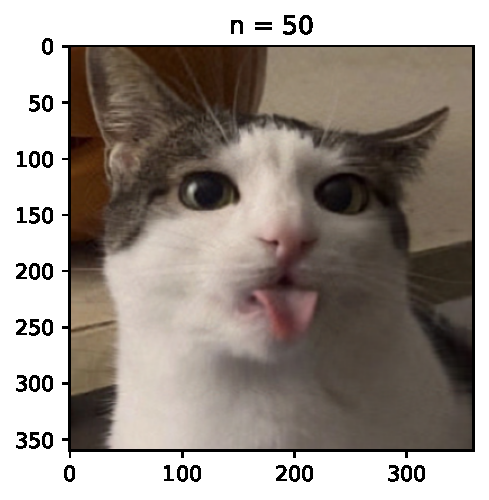
\includegraphics{day_14_files/figure-pdf/cell-21-output-1.pdf}

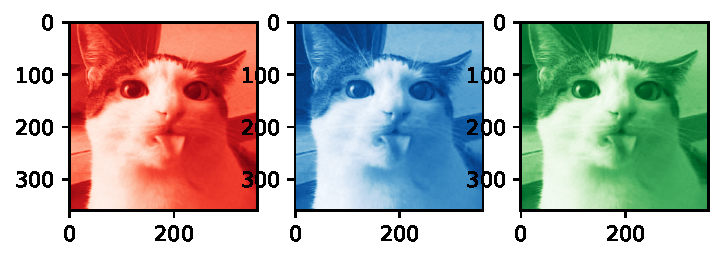
\includegraphics{day_14_files/figure-pdf/cell-21-output-2.pdf}

\subsection{\texorpdfstring{\emph{How many singular values to
keep?}}{How many singular values to keep?}}\label{how-many-singular-values-to-keep}

\begin{Shaded}
\begin{Highlighting}[]
\CommentTok{\# Plotting the singular values}
\NormalTok{plt.figure(figsize}\OperatorTok{=}\NormalTok{(}\DecValTok{8}\NormalTok{,}\DecValTok{4}\NormalTok{))}

\NormalTok{plt.subplot(}\DecValTok{1}\NormalTok{, }\DecValTok{2}\NormalTok{, }\DecValTok{1}\NormalTok{)}
\NormalTok{plt.plot(}\BuiltInTok{range}\NormalTok{(}\DecValTok{1}\NormalTok{, }\BuiltInTok{len}\NormalTok{(S) }\OperatorTok{+} \DecValTok{1}\NormalTok{), S)}
\NormalTok{plt.xlabel(}\StringTok{\textquotesingle{}Singular Value Index\textquotesingle{}}\NormalTok{)}
\NormalTok{plt.ylabel(}\StringTok{\textquotesingle{}Singular Value\textquotesingle{}}\NormalTok{)}
\NormalTok{plt.title(}\StringTok{\textquotesingle{}Singular Values\textquotesingle{}}\NormalTok{)}

\NormalTok{plt.subplot(}\DecValTok{1}\NormalTok{, }\DecValTok{2}\NormalTok{, }\DecValTok{2}\NormalTok{)}
\NormalTok{plt.plot(}\BuiltInTok{range}\NormalTok{(}\DecValTok{1}\NormalTok{, }\BuiltInTok{len}\NormalTok{(S) }\OperatorTok{+} \DecValTok{1}\NormalTok{), S)}
\NormalTok{plt.xlabel(}\StringTok{\textquotesingle{}Singular Value Index\textquotesingle{}}\NormalTok{)}
\NormalTok{plt.ylabel(}\StringTok{\textquotesingle{}Singular Value (log scale)\textquotesingle{}}\NormalTok{)}
\NormalTok{plt.title(}\StringTok{\textquotesingle{}Singular Values (log scale)\textquotesingle{}}\NormalTok{)}
\NormalTok{plt.yscale(}\StringTok{\textquotesingle{}log\textquotesingle{}}\NormalTok{)}

\NormalTok{plt.tight\_layout()}
\NormalTok{plt.show()}
\end{Highlighting}
\end{Shaded}

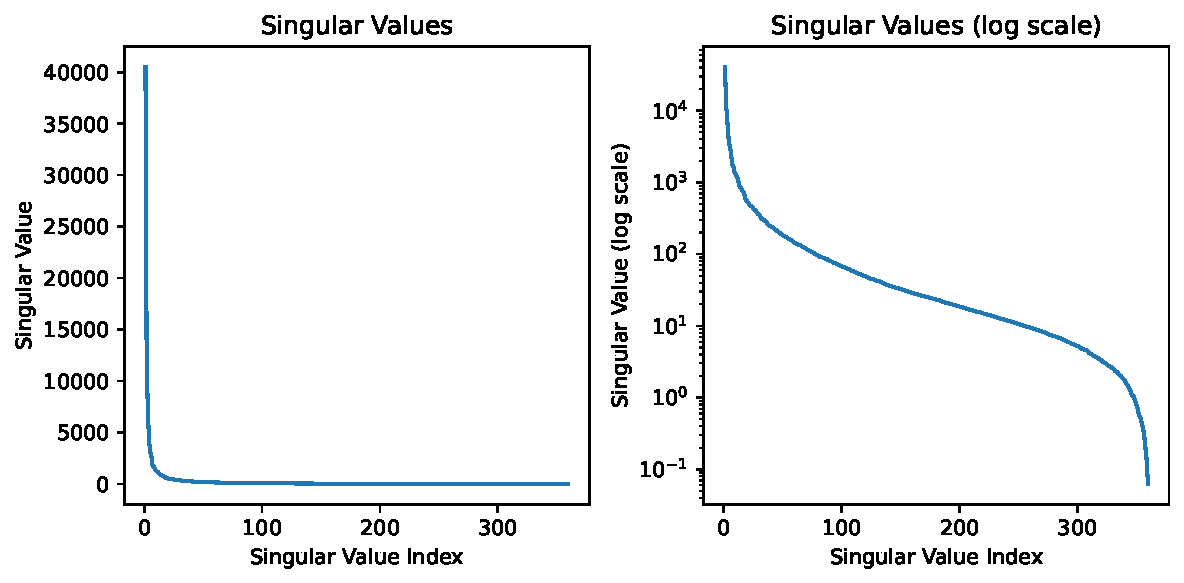
\includegraphics{day_14_files/figure-pdf/cell-22-output-1.pdf}

\subsection{\texorpdfstring{\emph{Different sorts of
images}}{Different sorts of images}}\label{different-sorts-of-images}

Just plain noise:

\begin{Shaded}
\begin{Highlighting}[]
\NormalTok{noise }\OperatorTok{=}\NormalTok{ np.random.randint(}\DecValTok{0}\NormalTok{,}\DecValTok{2}\NormalTok{,size}\OperatorTok{=}\NormalTok{(}\DecValTok{200}\NormalTok{,}\DecValTok{200}\NormalTok{))}
\NormalTok{plt.imshow(noise, cmap}\OperatorTok{=}\StringTok{\textquotesingle{}gray\textquotesingle{}}\NormalTok{)}
\end{Highlighting}
\end{Shaded}

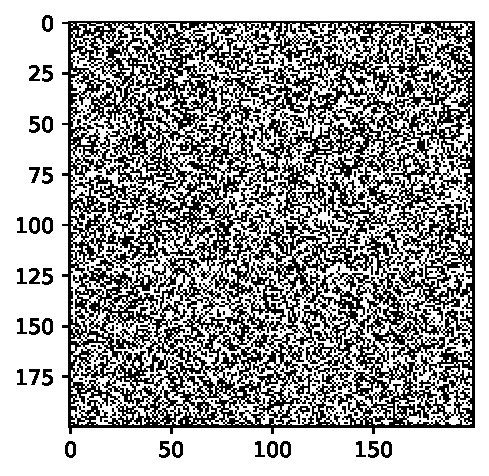
\includegraphics{day_14_files/figure-pdf/cell-23-output-1.pdf}

\subsection{\texorpdfstring{\emph{}}{}}\label{section-2}

\begin{Shaded}
\begin{Highlighting}[]
\NormalTok{U\_N, S\_N, Vt\_N }\OperatorTok{=}\NormalTok{ np.linalg.svd(noise, full\_matrices}\OperatorTok{=}\VariableTok{False}\NormalTok{)}

\CommentTok{\# Plotting the compressed noise for different values of n}
\NormalTok{components }\OperatorTok{=}\NormalTok{ [}\DecValTok{1}\NormalTok{, }\DecValTok{5}\NormalTok{, }\DecValTok{10}\NormalTok{, }\DecValTok{50}\NormalTok{, }\DecValTok{100}\NormalTok{, }\DecValTok{200}\NormalTok{]}

\NormalTok{fig }\OperatorTok{=}\NormalTok{ plt.figure(figsize}\OperatorTok{=}\NormalTok{(}\DecValTok{12}\NormalTok{,}\DecValTok{8}\NormalTok{))}

\ControlFlowTok{for}\NormalTok{ i }\KeywordTok{in} \BuiltInTok{range}\NormalTok{(}\BuiltInTok{len}\NormalTok{(components)):}
\NormalTok{    plt.subplot(}\DecValTok{2}\NormalTok{, }\DecValTok{3}\NormalTok{, i}\OperatorTok{+}\DecValTok{1}\NormalTok{)}
\NormalTok{    noise\_compressed }\OperatorTok{=}\NormalTok{ np.matrix(U\_N[:, :components[i]]) }\OperatorTok{*}\NormalTok{ np.diag(S\_N[:components[i]]) }\OperatorTok{*}\NormalTok{ np.matrix(Vt\_N[:components[i], :])}
\NormalTok{    plt.imshow(noise\_compressed, cmap}\OperatorTok{=}\StringTok{\textquotesingle{}gray\textquotesingle{}}\NormalTok{)}
\NormalTok{    plt.title(}\StringTok{\textquotesingle{}n = }\SpecialCharTok{\%s}\StringTok{\textquotesingle{}} \OperatorTok{\%}\NormalTok{ components[i])}

\NormalTok{plt.tight\_layout()}
\NormalTok{plt.show()}
\end{Highlighting}
\end{Shaded}

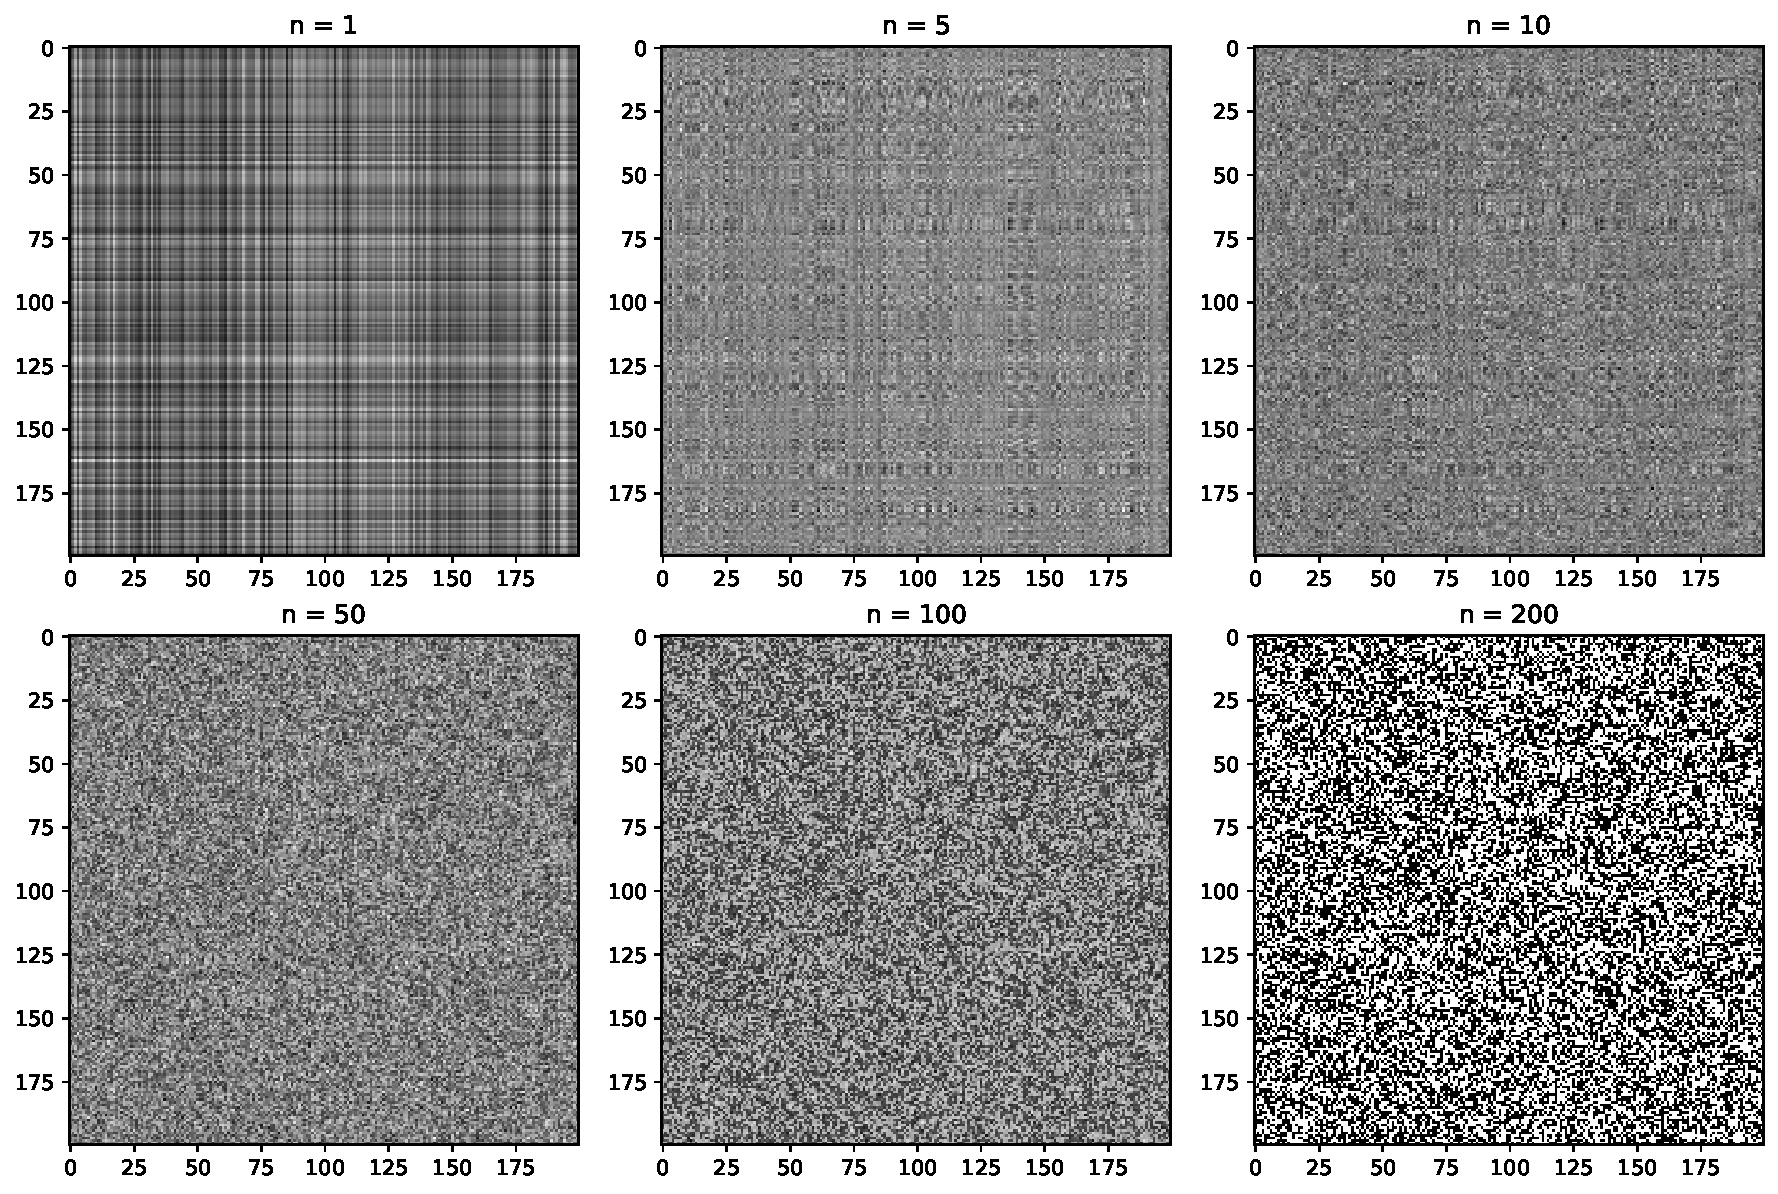
\includegraphics{day_14_files/figure-pdf/cell-24-output-1.pdf}

\subsection{\texorpdfstring{\emph{}}{}}\label{section-3}

\begin{Shaded}
\begin{Highlighting}[]
\KeywordTok{def}\NormalTok{ plot\_singular\_values(S, title):}
\NormalTok{    plt.plot(}\BuiltInTok{range}\NormalTok{(}\DecValTok{1}\NormalTok{, }\BuiltInTok{len}\NormalTok{(S) }\OperatorTok{+} \DecValTok{1}\NormalTok{), S)}
\NormalTok{    plt.xlabel(}\StringTok{\textquotesingle{}Singular Value Index\textquotesingle{}}\NormalTok{)}
\NormalTok{    plt.ylabel(}\StringTok{\textquotesingle{}Singular Value\textquotesingle{}}\NormalTok{)}
\NormalTok{    plt.title(title)}

\NormalTok{plt.figure(figsize}\OperatorTok{=}\NormalTok{(}\DecValTok{8}\NormalTok{, }\DecValTok{8}\NormalTok{))}

\NormalTok{plt.subplot(}\DecValTok{2}\NormalTok{, }\DecValTok{2}\NormalTok{, }\DecValTok{1}\NormalTok{)}
\NormalTok{plot\_singular\_values(S\_N, }\StringTok{\textquotesingle{}Singular Values\textquotesingle{}}\NormalTok{)}

\NormalTok{plt.subplot(}\DecValTok{2}\NormalTok{, }\DecValTok{2}\NormalTok{, }\DecValTok{2}\NormalTok{)}
\NormalTok{plot\_singular\_values(S\_N, }\StringTok{\textquotesingle{}Singular Values (log scale)\textquotesingle{}}\NormalTok{)}
\NormalTok{plt.yscale(}\StringTok{\textquotesingle{}log\textquotesingle{}}\NormalTok{)}

\NormalTok{plt.subplot(}\DecValTok{2}\NormalTok{, }\DecValTok{2}\NormalTok{, }\DecValTok{3}\NormalTok{)}
\NormalTok{plot\_singular\_values(S\_N[}\DecValTok{1}\NormalTok{:], }\StringTok{\textquotesingle{}Singular Values (without first singular value)\textquotesingle{}}\NormalTok{)}

\NormalTok{plt.subplot(}\DecValTok{2}\NormalTok{, }\DecValTok{2}\NormalTok{, }\DecValTok{4}\NormalTok{)}
\NormalTok{plot\_singular\_values(S\_N[}\DecValTok{1}\NormalTok{:], }\StringTok{\textquotesingle{}Singular Values (without first singular value, log scale)\textquotesingle{}}\NormalTok{)}
\NormalTok{plt.yscale(}\StringTok{\textquotesingle{}log\textquotesingle{}}\NormalTok{)}

\NormalTok{plt.tight\_layout()}
\NormalTok{plt.show()}
\end{Highlighting}
\end{Shaded}

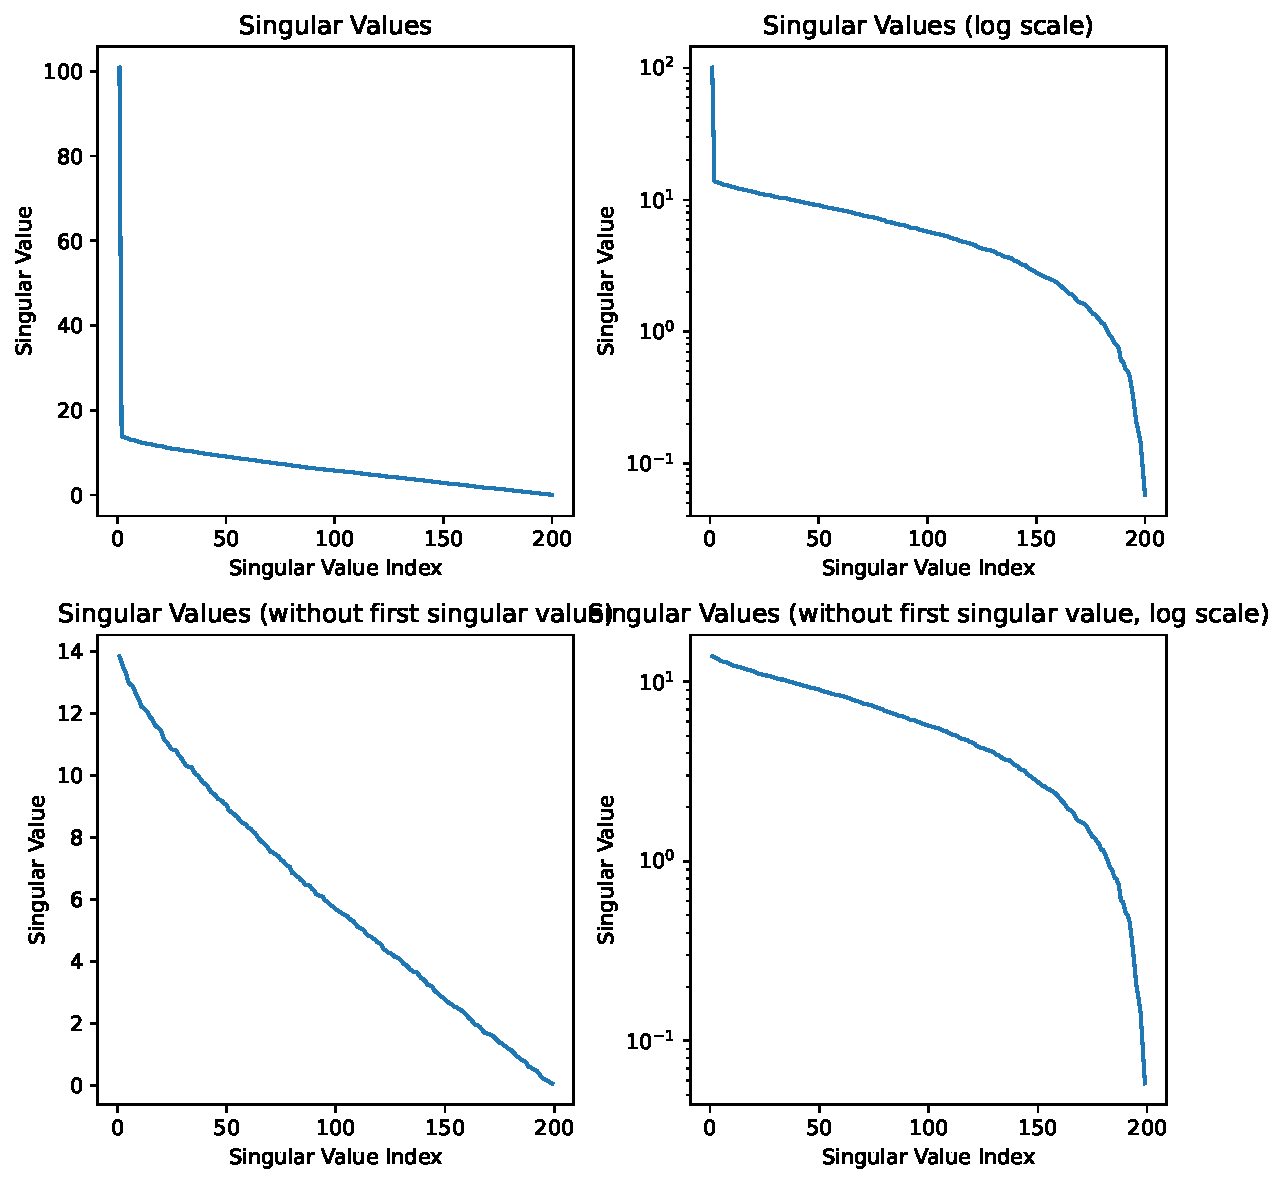
\includegraphics{day_14_files/figure-pdf/cell-25-output-1.pdf}

\subsection{\texorpdfstring{\emph{Plaid
shirt}}{Plaid shirt}}\label{plaid-shirt}

\begin{Shaded}
\begin{Highlighting}[]
\CommentTok{\# Show plaid pattern image}
\NormalTok{plaid\_image }\OperatorTok{=}\NormalTok{ cv2.imread(}\StringTok{\textquotesingle{}plaid\_pattern.jpg\textquotesingle{}}\NormalTok{)}
\NormalTok{plt.imshow(plaid\_image[:,:,::}\OperatorTok{{-}}\DecValTok{1}\NormalTok{])}
\NormalTok{plt.title(}\StringTok{\textquotesingle{}Plaid Pattern Image\textquotesingle{}}\NormalTok{)}
\NormalTok{plt.show()}

\CommentTok{\# Split the image into R, G, and B color channels}
\NormalTok{B, G, R }\OperatorTok{=}\NormalTok{ cv2.split(plaid\_image)}
\NormalTok{plt.subplot(}\DecValTok{1}\NormalTok{, }\DecValTok{3}\NormalTok{, }\DecValTok{1}\NormalTok{)}
\NormalTok{plt.imshow(R, cmap}\OperatorTok{=}\StringTok{\textquotesingle{}Reds\_r\textquotesingle{}}\NormalTok{)}
\NormalTok{plt.subplot(}\DecValTok{1}\NormalTok{, }\DecValTok{3}\NormalTok{, }\DecValTok{2}\NormalTok{)}
\NormalTok{plt.imshow(B, cmap}\OperatorTok{=}\StringTok{\textquotesingle{}Blues\_r\textquotesingle{}}\NormalTok{)}
\NormalTok{plt.subplot(}\DecValTok{1}\NormalTok{, }\DecValTok{3}\NormalTok{, }\DecValTok{3}\NormalTok{)}
\NormalTok{plt.imshow(G, cmap}\OperatorTok{=}\StringTok{\textquotesingle{}Greens\_r\textquotesingle{}}\NormalTok{)}
\NormalTok{plt.show()}
\end{Highlighting}
\end{Shaded}

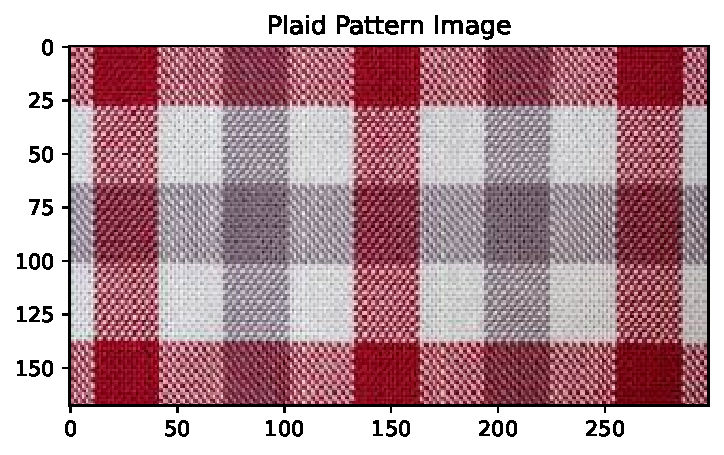
\includegraphics{day_14_files/figure-pdf/cell-26-output-1.pdf}

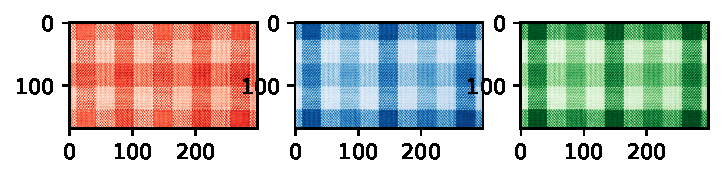
\includegraphics{day_14_files/figure-pdf/cell-26-output-2.pdf}

\subsection{\texorpdfstring{\emph{}}{}}\label{section-4}

\begin{Shaded}
\begin{Highlighting}[]
\KeywordTok{def}\NormalTok{ rgb\_approximation(R, G, B, n):}
\NormalTok{    U\_R, S\_R, Vt\_R }\OperatorTok{=}\NormalTok{ np.linalg.svd(R, full\_matrices}\OperatorTok{=}\VariableTok{False}\NormalTok{)}
\NormalTok{    U\_G, S\_G, Vt\_G }\OperatorTok{=}\NormalTok{ np.linalg.svd(G, full\_matrices}\OperatorTok{=}\VariableTok{False}\NormalTok{)}
\NormalTok{    U\_B, S\_B, Vt\_B }\OperatorTok{=}\NormalTok{ np.linalg.svd(B, full\_matrices}\OperatorTok{=}\VariableTok{False}\NormalTok{)}

\NormalTok{    R\_compressed }\OperatorTok{=}\NormalTok{ np.matrix(U\_R[:, :n]) }\OperatorTok{*}\NormalTok{ np.diag(S\_R[:n]) }\OperatorTok{*}\NormalTok{ np.matrix(Vt\_R[:n, :])}
\NormalTok{    G\_compressed }\OperatorTok{=}\NormalTok{ np.matrix(U\_G[:, :n]) }\OperatorTok{*}\NormalTok{ np.diag(S\_G[:n]) }\OperatorTok{*}\NormalTok{ np.matrix(Vt\_G[:n, :])}
\NormalTok{    B\_compressed }\OperatorTok{=}\NormalTok{ np.matrix(U\_B[:, :n]) }\OperatorTok{*}\NormalTok{ np.diag(S\_B[:n]) }\OperatorTok{*}\NormalTok{ np.matrix(Vt\_B[:n, :])}

\NormalTok{    compressed\_image }\OperatorTok{=}\NormalTok{ cv2.merge([np.clip(R\_compressed, }\DecValTok{1}\NormalTok{, }\DecValTok{255}\NormalTok{), np.clip(G\_compressed, }\DecValTok{1}\NormalTok{, }\DecValTok{255}\NormalTok{), np.clip(B\_compressed, }\DecValTok{1}\NormalTok{, }\DecValTok{255}\NormalTok{)])}
\NormalTok{    compressed\_image }\OperatorTok{=}\NormalTok{ compressed\_image.astype(np.uint8)}

    \ControlFlowTok{return}\NormalTok{ compressed\_image}

\NormalTok{n\_values }\OperatorTok{=}\NormalTok{ [}\DecValTok{1}\NormalTok{, }\DecValTok{5}\NormalTok{, }\DecValTok{25}\NormalTok{]}

\NormalTok{plt.figure(figsize}\OperatorTok{=}\NormalTok{(}\DecValTok{12}\NormalTok{, }\DecValTok{6}\NormalTok{))}
\ControlFlowTok{for}\NormalTok{ i, n }\KeywordTok{in} \BuiltInTok{enumerate}\NormalTok{(n\_values):}
\NormalTok{    plt.subplot(}\DecValTok{1}\NormalTok{, }\BuiltInTok{len}\NormalTok{(n\_values), i}\OperatorTok{+}\DecValTok{1}\NormalTok{)}
\NormalTok{    plt.imshow(rgb\_approximation(R, G, B, n))}
\NormalTok{    plt.title(}\StringTok{\textquotesingle{}n = }\SpecialCharTok{\%s}\StringTok{\textquotesingle{}} \OperatorTok{\%}\NormalTok{ n)}

\NormalTok{plt.tight\_layout()}
\NormalTok{plt.show()}
\end{Highlighting}
\end{Shaded}

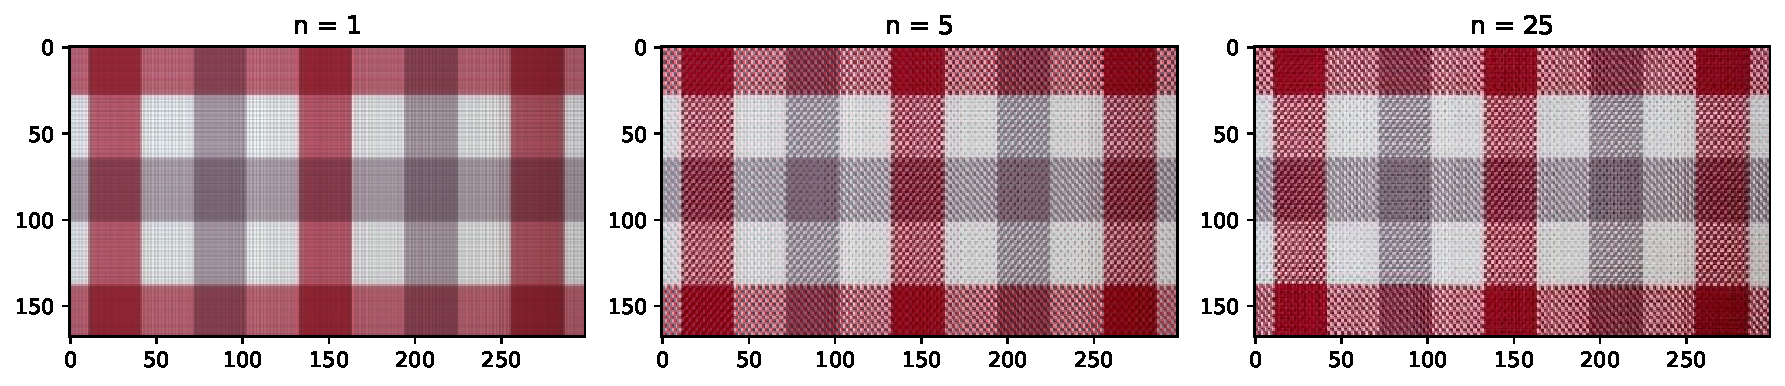
\includegraphics{day_14_files/figure-pdf/cell-27-output-1.pdf}

\subsection{\texorpdfstring{\emph{Singular
values}}{Singular values}}\label{singular-values}

\begin{Shaded}
\begin{Highlighting}[]
\NormalTok{plt.figure(figsize}\OperatorTok{=}\NormalTok{(}\DecValTok{12}\NormalTok{, }\DecValTok{8}\NormalTok{))}

\NormalTok{plt.subplot(}\DecValTok{2}\NormalTok{, }\DecValTok{3}\NormalTok{, }\DecValTok{1}\NormalTok{)}
\NormalTok{plot\_singular\_values(S\_R, }\StringTok{\textquotesingle{}Singular Values (R)\textquotesingle{}}\NormalTok{)}

\NormalTok{plt.subplot(}\DecValTok{2}\NormalTok{, }\DecValTok{3}\NormalTok{, }\DecValTok{2}\NormalTok{)}
\NormalTok{plot\_singular\_values(S\_G, }\StringTok{\textquotesingle{}Singular Values (G)\textquotesingle{}}\NormalTok{)}

\NormalTok{plt.subplot(}\DecValTok{2}\NormalTok{, }\DecValTok{3}\NormalTok{, }\DecValTok{3}\NormalTok{)}
\NormalTok{plot\_singular\_values(S\_B, }\StringTok{\textquotesingle{}Singular Values (B)\textquotesingle{}}\NormalTok{)}

\NormalTok{plt.subplot(}\DecValTok{2}\NormalTok{, }\DecValTok{3}\NormalTok{, }\DecValTok{4}\NormalTok{)}
\NormalTok{plot\_singular\_values(S\_R, }\StringTok{\textquotesingle{}Singular Values (log scale) (R)\textquotesingle{}}\NormalTok{)}
\NormalTok{plt.yscale(}\StringTok{\textquotesingle{}log\textquotesingle{}}\NormalTok{)}

\NormalTok{plt.subplot(}\DecValTok{2}\NormalTok{, }\DecValTok{3}\NormalTok{, }\DecValTok{5}\NormalTok{)}
\NormalTok{plot\_singular\_values(S\_G, }\StringTok{\textquotesingle{}Singular Values (log scale) (G)\textquotesingle{}}\NormalTok{)}
\NormalTok{plt.yscale(}\StringTok{\textquotesingle{}log\textquotesingle{}}\NormalTok{)}

\NormalTok{plt.subplot(}\DecValTok{2}\NormalTok{, }\DecValTok{3}\NormalTok{, }\DecValTok{6}\NormalTok{)}
\NormalTok{plot\_singular\_values(S\_B, }\StringTok{\textquotesingle{}Singular Values (log scale) (B)\textquotesingle{}}\NormalTok{)}
\NormalTok{plt.yscale(}\StringTok{\textquotesingle{}log\textquotesingle{}}\NormalTok{)}

\NormalTok{plt.tight\_layout()}
\NormalTok{plt.show()}
\end{Highlighting}
\end{Shaded}

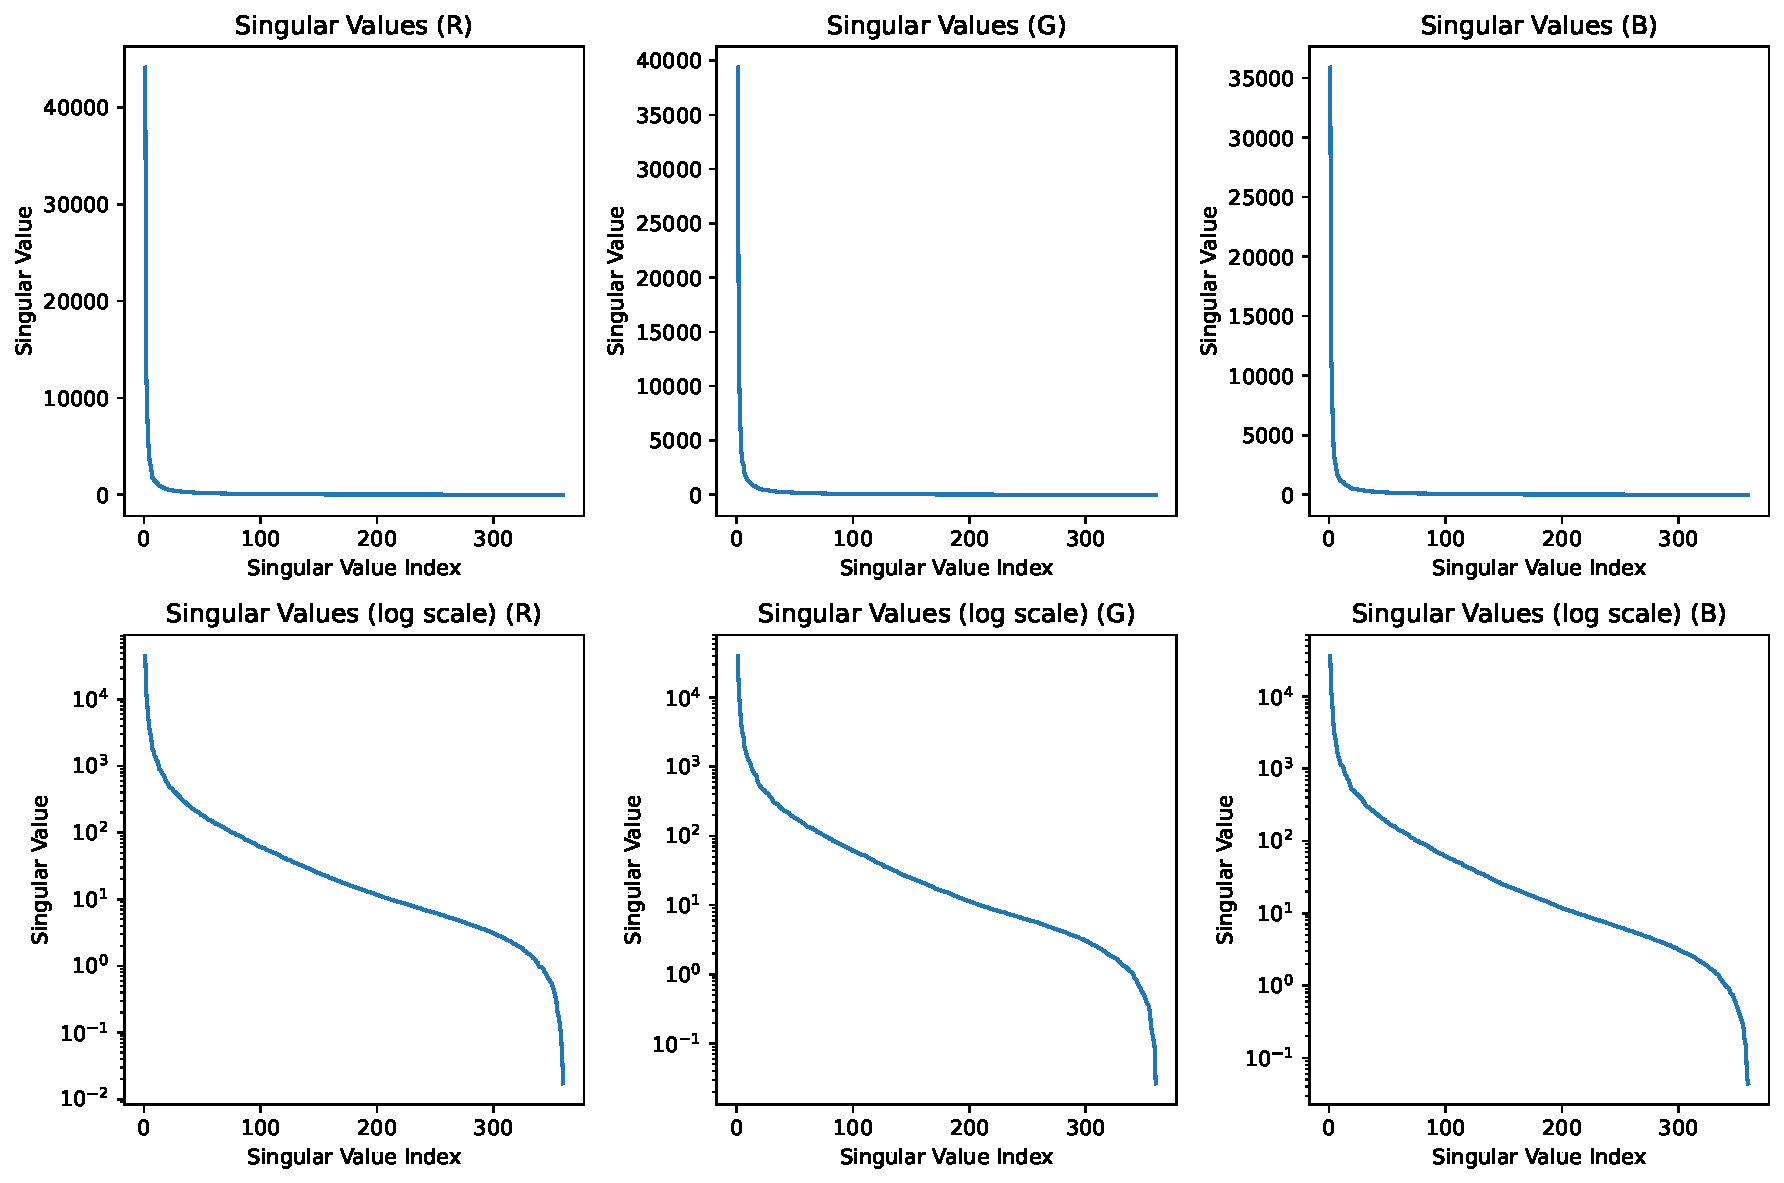
\includegraphics{day_14_files/figure-pdf/cell-28-output-1.pdf}

\subsection{\texorpdfstring{\emph{Individual
components}}{Individual components}}\label{individual-components}

First component:

\begin{Shaded}
\begin{Highlighting}[]
\NormalTok{ U\_R, S\_R, Vt\_R }\OperatorTok{=}\NormalTok{ np.linalg.svd(R, full\_matrices}\OperatorTok{=}\VariableTok{False}\NormalTok{)}
\NormalTok{plot\_uv(}\DecValTok{0}\NormalTok{, U}\OperatorTok{=}\NormalTok{U\_R, S}\OperatorTok{=}\NormalTok{S\_R, Vt}\OperatorTok{=}\NormalTok{Vt\_R)}
\end{Highlighting}
\end{Shaded}

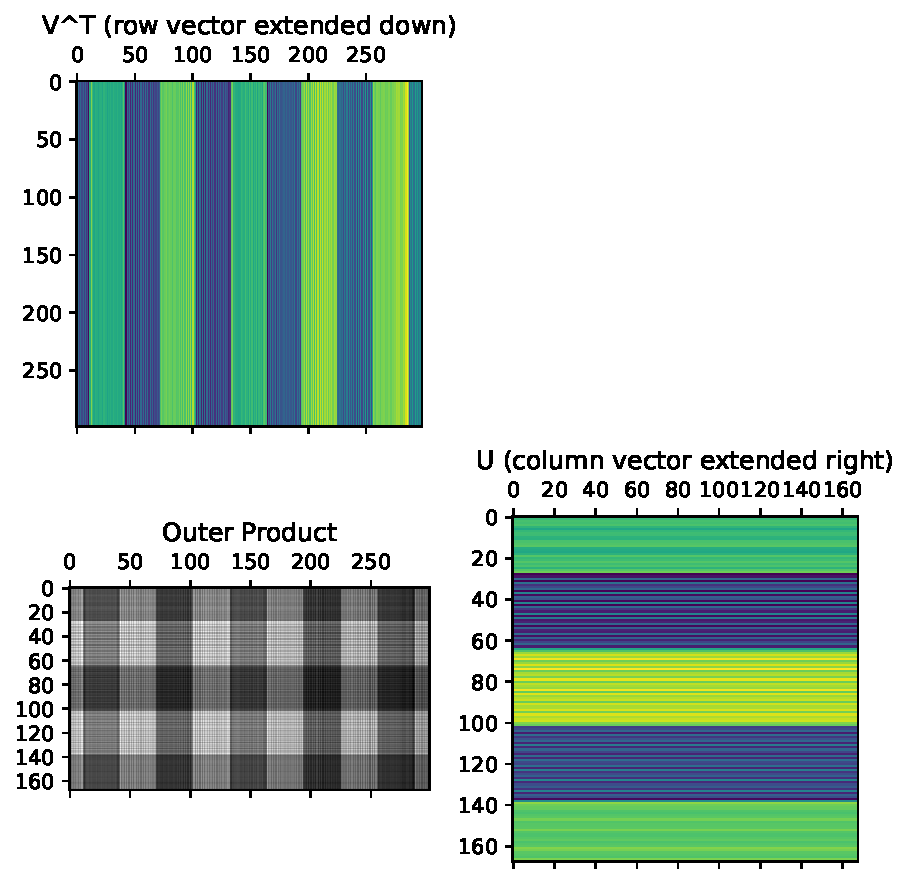
\includegraphics{day_14_files/figure-pdf/cell-29-output-1.pdf}

\subsection{\texorpdfstring{\emph{}}{}}\label{section-5}

Second component:

\begin{Shaded}
\begin{Highlighting}[]
\NormalTok{plot\_uv(}\DecValTok{1}\NormalTok{, U}\OperatorTok{=}\NormalTok{U\_R, S}\OperatorTok{=}\NormalTok{S\_R, Vt}\OperatorTok{=}\NormalTok{Vt\_R)}
\end{Highlighting}
\end{Shaded}

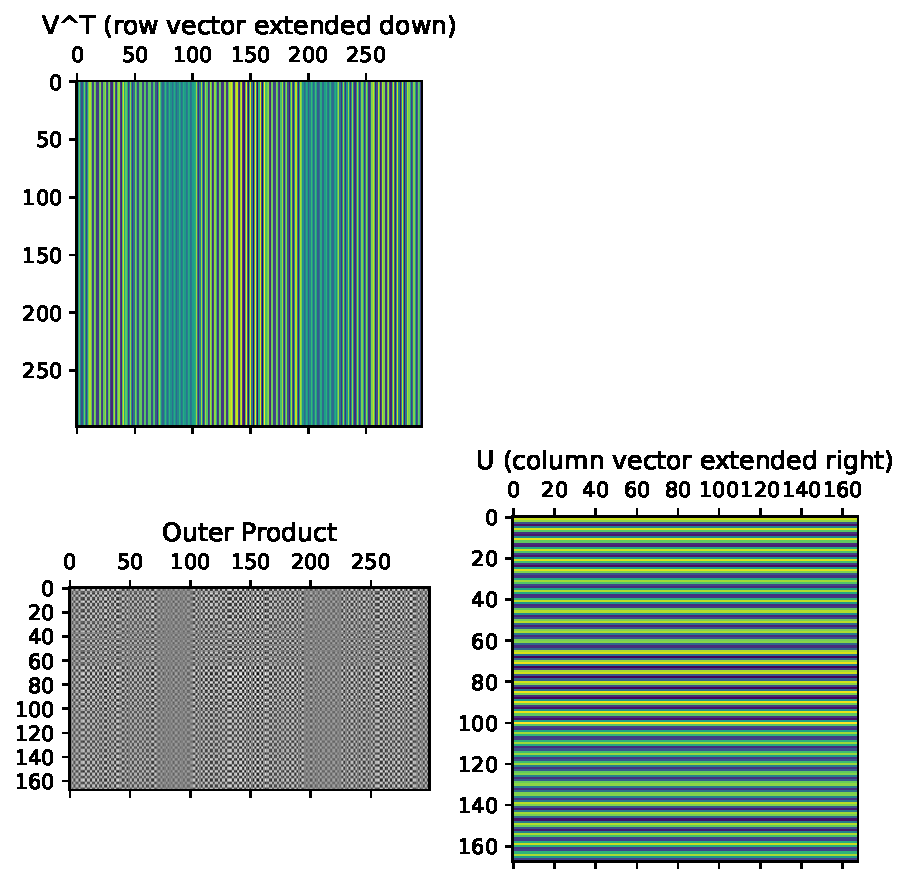
\includegraphics{day_14_files/figure-pdf/cell-30-output-1.pdf}

\subsection{\texorpdfstring{\emph{Using ``PCA'' from
sklearn}}{Using ``PCA'' from sklearn}}\label{using-pca-from-sklearn}

This is just an easier way to implement taking these first few
components\ldots{}

\begin{Shaded}
\begin{Highlighting}[]
\ImportTok{from}\NormalTok{ sklearn.decomposition }\ImportTok{import}\NormalTok{ PCA}
\NormalTok{pca }\OperatorTok{=}\NormalTok{ PCA(n\_components}\OperatorTok{=}\DecValTok{2}\NormalTok{)}
\NormalTok{pca.fit(R) }\CommentTok{\# fit the model {-}{-} compute the matrices}
\NormalTok{transformed }\OperatorTok{=}\NormalTok{ pca.transform(R) }\CommentTok{\# transform the data}
\BuiltInTok{print}\NormalTok{(}\SpecialStringTok{f\textquotesingle{}The shape of the image is }\SpecialCharTok{\{}\NormalTok{R}\SpecialCharTok{.}\NormalTok{shape}\SpecialCharTok{\}}\SpecialStringTok{, and the shape of the compressed image is }\SpecialCharTok{\{}\NormalTok{transformed}\SpecialCharTok{.}\NormalTok{shape}\SpecialCharTok{\}}\SpecialStringTok{\textquotesingle{}}\NormalTok{)}
\NormalTok{plt.imshow(transformed.T)}
\end{Highlighting}
\end{Shaded}

\begin{verbatim}
The shape of the image is (168, 299), and the shape of the compressed image is (168, 2)
\end{verbatim}

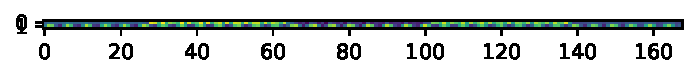
\includegraphics{day_14_files/figure-pdf/cell-31-output-2.pdf}

. . .

\begin{Shaded}
\begin{Highlighting}[]
\NormalTok{plt.imshow(pca.inverse\_transform(transformed))}
\end{Highlighting}
\end{Shaded}

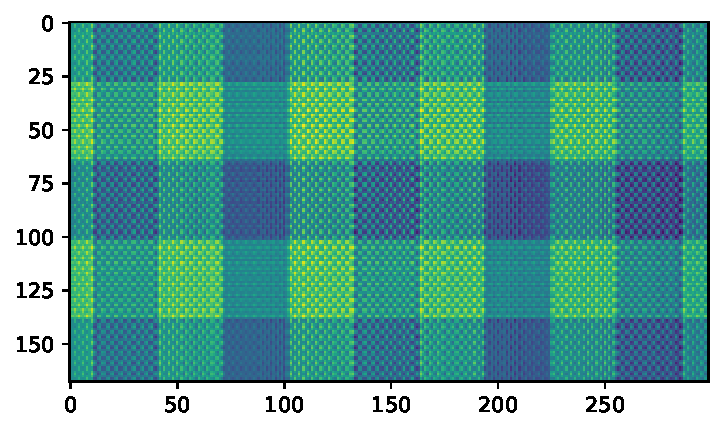
\includegraphics{day_14_files/figure-pdf/cell-32-output-1.pdf}

\subsection{\texorpdfstring{\emph{}}{}}\label{section-6}

Try adding noise\ldots{}

\begin{Shaded}
\begin{Highlighting}[]
\NormalTok{alpha }\OperatorTok{=} \DecValTok{10}
\NormalTok{R\_noisy }\OperatorTok{=}\NormalTok{ R }\OperatorTok{+}\NormalTok{ np.random.normal(}\DecValTok{0}\NormalTok{, }\DecValTok{10}\NormalTok{, R.shape)}\OperatorTok{*}\NormalTok{alpha}
\NormalTok{plt.imshow(R\_noisy)}
\end{Highlighting}
\end{Shaded}

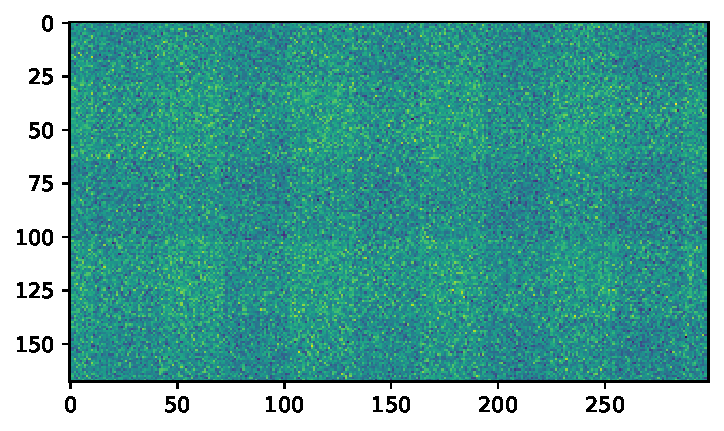
\includegraphics{day_14_files/figure-pdf/cell-33-output-1.pdf}

Now clean it up with PCA:

\begin{Shaded}
\begin{Highlighting}[]
\NormalTok{pca }\OperatorTok{=}\NormalTok{ PCA(n\_components}\OperatorTok{=}\DecValTok{2}\NormalTok{)}
\NormalTok{pca.fit(R\_noisy)}
\NormalTok{plt.imshow(pca.inverse\_transform(pca.transform(R\_noisy)))}
\end{Highlighting}
\end{Shaded}

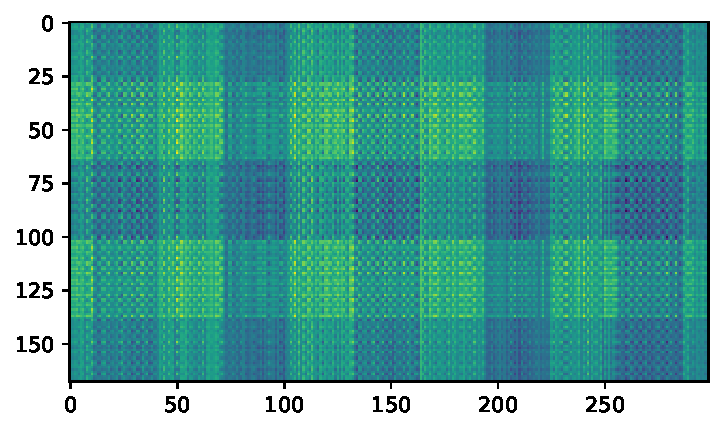
\includegraphics{day_14_files/figure-pdf/cell-34-output-1.pdf}

\subsection{\texorpdfstring{\emph{Skills}}{Skills}}\label{skills-1}

\begin{itemize}
\tightlist
\item
  Compute the SVD of an image matrix and interpret \(U\), \(S\), \(V\)
\item
  Reconstruct an image from the first \(n\) singular value components
\item
  Apply SVD to color images (per channel)
\item
  Use PCA as a convenient truncated SVD; interpret variance captured
\end{itemize}

\section{\texorpdfstring{\emph{SVD in higher
dimensions}}{SVD in higher dimensions}}\label{svd-in-higher-dimensions}

PCA on high-dimensional data (faces); low-rank reconstruction;
connection to SVD.

\subsection{\texorpdfstring{\emph{Faces}}{Faces}}\label{faces}

\begin{Shaded}
\begin{Highlighting}[]
\ImportTok{from}\NormalTok{ sklearn.datasets }\ImportTok{import}\NormalTok{ fetch\_lfw\_people}
\NormalTok{faces }\OperatorTok{=}\NormalTok{ fetch\_lfw\_people(min\_faces\_per\_person}\OperatorTok{=}\DecValTok{60}\NormalTok{)}


\CommentTok{\# display a few of the faces, along with their names}
\NormalTok{fig, ax }\OperatorTok{=}\NormalTok{ plt.subplots(}\DecValTok{3}\NormalTok{, }\DecValTok{4}\NormalTok{)}
\ControlFlowTok{for}\NormalTok{ i, axi }\KeywordTok{in} \BuiltInTok{enumerate}\NormalTok{(ax.flat):}
\NormalTok{    axi.imshow(faces.images[i], cmap}\OperatorTok{=}\StringTok{\textquotesingle{}bone\textquotesingle{}}\NormalTok{)}
\NormalTok{    axi.}\BuiltInTok{set}\NormalTok{(xticks}\OperatorTok{=}\NormalTok{[], yticks}\OperatorTok{=}\NormalTok{[],}
\NormalTok{            xlabel}\OperatorTok{=}\NormalTok{faces.target\_names[faces.target[i]]) }

\BuiltInTok{print}\NormalTok{(}\SpecialStringTok{f\textquotesingle{}The shape of the faces dataset is }\SpecialCharTok{\{}\NormalTok{faces}\SpecialCharTok{.}\NormalTok{images}\SpecialCharTok{.}\NormalTok{shape}\SpecialCharTok{\}}\SpecialStringTok{\textquotesingle{}}\NormalTok{)}
\end{Highlighting}
\end{Shaded}

\begin{verbatim}
The shape of the faces dataset is (1348, 62, 47)
\end{verbatim}

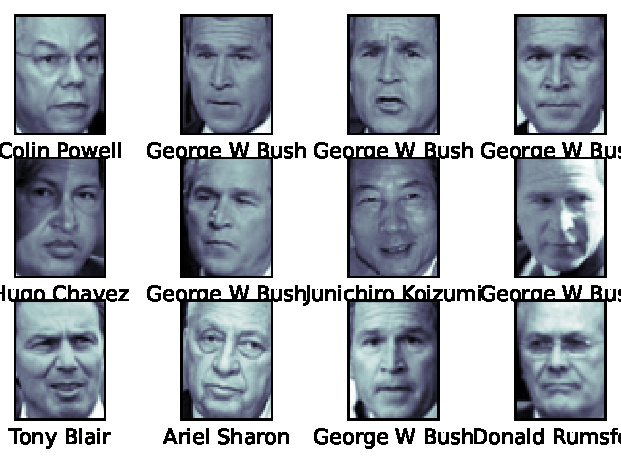
\includegraphics{day_14_files/figure-pdf/cell-35-output-2.pdf}

\subsection{\texorpdfstring{\emph{PCA on
faces}}{PCA on faces}}\label{pca-on-faces}

\begin{Shaded}
\begin{Highlighting}[]
\NormalTok{pca }\OperatorTok{=}\NormalTok{ PCA(}\DecValTok{150}\NormalTok{, svd\_solver}\OperatorTok{=}\StringTok{\textquotesingle{}randomized\textquotesingle{}}\NormalTok{, random\_state}\OperatorTok{=}\DecValTok{42}\NormalTok{)}
\NormalTok{pca\_small }\OperatorTok{=}\NormalTok{ PCA(}\DecValTok{10}\NormalTok{, svd\_solver}\OperatorTok{=}\StringTok{\textquotesingle{}randomized\textquotesingle{}}\NormalTok{, random\_state}\OperatorTok{=}\DecValTok{42}\NormalTok{)}
\NormalTok{pca\_very\_small }\OperatorTok{=}\NormalTok{ PCA(}\DecValTok{2}\NormalTok{, svd\_solver}\OperatorTok{=}\StringTok{\textquotesingle{}randomized\textquotesingle{}}\NormalTok{, random\_state}\OperatorTok{=}\DecValTok{42}\NormalTok{)}
\NormalTok{pca.fit(faces.data)}
\NormalTok{pca\_small.fit(faces.data)}
\NormalTok{pca\_very\_small.fit(faces.data)}
\end{Highlighting}
\end{Shaded}

\begin{verbatim}
PCA(n_components=2, random_state=42, svd_solver='randomized')
\end{verbatim}

\marginnote{\begin{footnotesize}

This treatment from
\href{https://github.com/jakevdp/PythonDataScienceHandbook/blob/master/notebooks/05.09-Principal-Component-Analysis.ipynb}{here}

\end{footnotesize}}

. . .

\begin{Shaded}
\begin{Highlighting}[]
\NormalTok{fig, axes }\OperatorTok{=}\NormalTok{ plt.subplots(}\DecValTok{3}\NormalTok{, }\DecValTok{8}\NormalTok{, figsize}\OperatorTok{=}\NormalTok{(}\DecValTok{9}\NormalTok{, }\DecValTok{4}\NormalTok{),}
\NormalTok{                         subplot\_kw}\OperatorTok{=}\NormalTok{\{}\StringTok{\textquotesingle{}xticks\textquotesingle{}}\NormalTok{:[], }\StringTok{\textquotesingle{}yticks\textquotesingle{}}\NormalTok{:[]\},}
\NormalTok{                         gridspec\_kw}\OperatorTok{=}\BuiltInTok{dict}\NormalTok{(hspace}\OperatorTok{=}\FloatTok{0.1}\NormalTok{, wspace}\OperatorTok{=}\FloatTok{0.1}\NormalTok{))}
\ControlFlowTok{for}\NormalTok{ i, ax }\KeywordTok{in} \BuiltInTok{enumerate}\NormalTok{(axes.flat):}
\NormalTok{    ax.imshow(pca.components\_[i].reshape(}\DecValTok{62}\NormalTok{, }\DecValTok{47}\NormalTok{), cmap}\OperatorTok{=}\StringTok{\textquotesingle{}bone\textquotesingle{}}\NormalTok{)}
\end{Highlighting}
\end{Shaded}

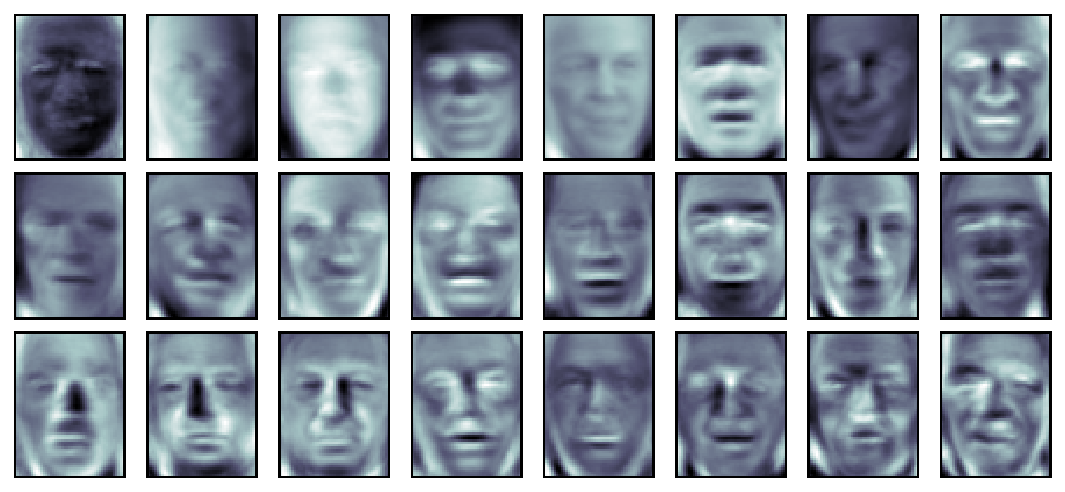
\includegraphics{day_14_files/figure-pdf/cell-37-output-1.pdf}

\subsection{\texorpdfstring{\emph{Reconstructions}}{Reconstructions}}\label{reconstructions}

\begin{Shaded}
\begin{Highlighting}[]
\CommentTok{\# Compute the components and projected faces}
\NormalTok{pca }\OperatorTok{=}\NormalTok{ pca.fit(faces.data)}
\NormalTok{components }\OperatorTok{=}\NormalTok{ pca.transform(faces.data)}
\NormalTok{projected }\OperatorTok{=}\NormalTok{ pca.inverse\_transform(components)}

\NormalTok{components\_small }\OperatorTok{=}\NormalTok{ pca\_small.transform(faces.data)}
\NormalTok{projected\_small }\OperatorTok{=}\NormalTok{ pca\_small.inverse\_transform(components\_small)}


\NormalTok{components\_very\_small }\OperatorTok{=}\NormalTok{ pca\_very\_small.transform(faces.data)}
\NormalTok{projected\_very\_small }\OperatorTok{=}\NormalTok{ pca\_very\_small.inverse\_transform(components\_very\_small)}
\end{Highlighting}
\end{Shaded}

\subsection{\texorpdfstring{\emph{}}{}}\label{section-7}

\begin{Shaded}
\begin{Highlighting}[]
\CommentTok{\# Plot the results}
\NormalTok{fig, ax }\OperatorTok{=}\NormalTok{ plt.subplots(}\DecValTok{4}\NormalTok{, }\DecValTok{10}\NormalTok{, figsize}\OperatorTok{=}\NormalTok{(}\DecValTok{10}\NormalTok{, }\FloatTok{6.5}\NormalTok{),}
\NormalTok{                       subplot\_kw}\OperatorTok{=}\NormalTok{\{}\StringTok{\textquotesingle{}xticks\textquotesingle{}}\NormalTok{:[], }\StringTok{\textquotesingle{}yticks\textquotesingle{}}\NormalTok{:[]\},}
\NormalTok{                       gridspec\_kw}\OperatorTok{=}\BuiltInTok{dict}\NormalTok{(hspace}\OperatorTok{=}\FloatTok{0.1}\NormalTok{, wspace}\OperatorTok{=}\FloatTok{0.1}\NormalTok{))}
\ControlFlowTok{for}\NormalTok{ i }\KeywordTok{in} \BuiltInTok{range}\NormalTok{(}\DecValTok{10}\NormalTok{):}
\NormalTok{    ax[}\DecValTok{0}\NormalTok{, i].imshow(faces.data[i].reshape(}\DecValTok{62}\NormalTok{, }\DecValTok{47}\NormalTok{), cmap}\OperatorTok{=}\StringTok{\textquotesingle{}binary\_r\textquotesingle{}}\NormalTok{)}
\NormalTok{    ax[}\DecValTok{1}\NormalTok{, i].imshow(projected\_very\_small[i].reshape(}\DecValTok{62}\NormalTok{, }\DecValTok{47}\NormalTok{), cmap}\OperatorTok{=}\StringTok{\textquotesingle{}binary\_r\textquotesingle{}}\NormalTok{)}
\NormalTok{    ax[}\DecValTok{2}\NormalTok{, i].imshow(projected\_small[i].reshape(}\DecValTok{62}\NormalTok{, }\DecValTok{47}\NormalTok{), cmap}\OperatorTok{=}\StringTok{\textquotesingle{}binary\_r\textquotesingle{}}\NormalTok{)}
\NormalTok{    ax[}\DecValTok{3}\NormalTok{, i].imshow(projected[i].reshape(}\DecValTok{62}\NormalTok{, }\DecValTok{47}\NormalTok{), cmap}\OperatorTok{=}\StringTok{\textquotesingle{}binary\_r\textquotesingle{}}\NormalTok{)}
    
\NormalTok{ax[}\DecValTok{0}\NormalTok{, }\DecValTok{0}\NormalTok{].set\_ylabel(}\StringTok{\textquotesingle{}full{-}dim}\CharTok{\textbackslash{}n}\StringTok{input\textquotesingle{}}\NormalTok{)}
\NormalTok{ax[}\DecValTok{1}\NormalTok{, }\DecValTok{0}\NormalTok{].set\_ylabel(}\StringTok{\textquotesingle{}2{-}dim}\CharTok{\textbackslash{}n}\StringTok{reconstruction\textquotesingle{}}\NormalTok{)}\OperatorTok{;}
\NormalTok{ax[}\DecValTok{2}\NormalTok{, }\DecValTok{0}\NormalTok{].set\_ylabel(}\StringTok{\textquotesingle{}10{-}dim}\CharTok{\textbackslash{}n}\StringTok{reconstruction\textquotesingle{}}\NormalTok{)}\OperatorTok{;}
\NormalTok{ax[}\DecValTok{3}\NormalTok{, }\DecValTok{0}\NormalTok{].set\_ylabel(}\StringTok{\textquotesingle{}150{-}dim}\CharTok{\textbackslash{}n}\StringTok{reconstruction\textquotesingle{}}\NormalTok{)}\OperatorTok{;}
\end{Highlighting}
\end{Shaded}

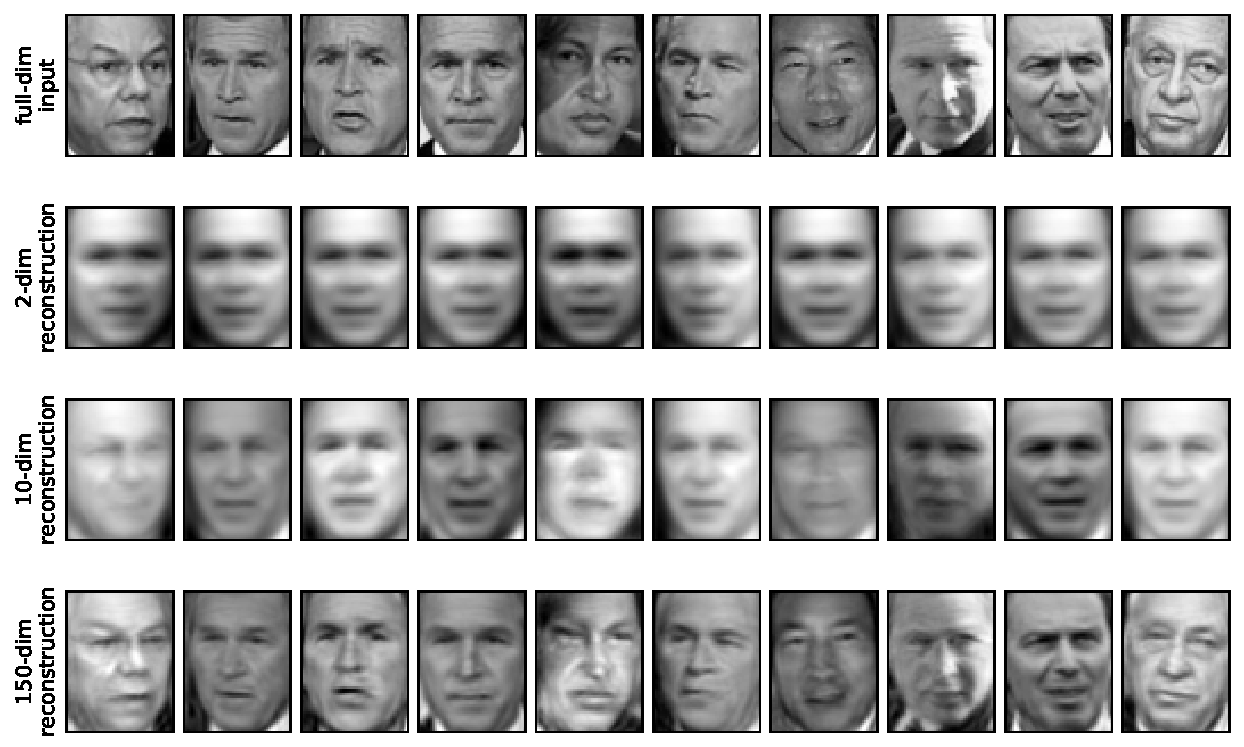
\includegraphics{day_14_files/figure-pdf/cell-39-output-1.pdf}

\subsection{\texorpdfstring{\emph{}}{}}\label{section-8}

Really cool demo of SVD image compression:
https://timbaumann.info/svd-image-compression-demo/

\subsection{\texorpdfstring{\emph{Skills}}{Skills}}\label{skills-2}

\begin{itemize}
\tightlist
\item
  Apply PCA to high-dimensional data (e.g., faces) and interpret
  components
\item
  Reconstruct data from a low-rank PCA approximation
\item
  Recognize PCA as truncated SVD on mean-centered data
\end{itemize}

\subsection{\texorpdfstring{\emph{Now you}}{Now you}}\label{now-you}

Code up your own image compression using SVD and show the left and right
singular vectors, the singular values, and the reconstructed images.

Share with the class!




\end{document}
